\documentclass[11pt,a4paper,oneside,openany]{report}
\usepackage{fontspec,xeCJK,geometry,xcolor,graphicx,amsmath,amssymb,array,booktabs,tabularx,fancyhdr,float,placeins,needspace,hyperref,fvextra}
\geometry{left=25mm,right=23mm,top=22mm,bottom=22mm,headheight=15pt,headsep=6mm}
\setmainfont{Times New Roman}\setsansfont{Segoe UI}\setmonofont{Consolas}
\setCJKmainfont[BoldFont=SimHei]{SimSun}\setCJKsansfont{Microsoft YaHei}\setCJKmonofont{Microsoft YaHei}
\definecolor{navy}{HTML}{203A4C}
\hypersetup{colorlinks=true,linkcolor=navy,urlcolor=navy,citecolor=navy,bookmarksnumbered=true,pdftitle={Verifiable Tutoring Lab: Executable Data, Preference Tuning, and Learner Memory},pdfauthor={Verifiable Tutoring Lab}}
\setcounter{tocdepth}{1}\setcounter{secnumdepth}{2}
\pagestyle{fancy}\fancyhf{}\fancyhead[L]{\small Verifiable Tutoring Lab}\fancyhead[R]{\small Technical Research Report}\fancyfoot[C]{\small\thepage}
\renewcommand{\headrulewidth}{0.3pt}
\setlength{\parindent}{0pt}\setlength{\parskip}{4pt}\linespread{1.06}
\setlength{\emergencystretch}{3em}
\clubpenalty=10000\widowpenalty=10000\displaywidowpenalty=10000
\setlength{\textfloatsep}{11pt}\setlength{\intextsep}{10pt}\setlength{\tabcolsep}{4.5pt}
\renewcommand{\topfraction}{0.9}\renewcommand{\bottomfraction}{0.8}\renewcommand{\textfraction}{0.08}\renewcommand{\floatpagefraction}{0.8}
\newcolumntype{Y}{>{\raggedright\arraybackslash}X}\renewcommand{\arraystretch}{1.14}\raggedbottom
\RecustomVerbatimEnvironment{verbatim}{Verbatim}{fontsize=\small,breaklines=true,breakanywhere=true,breaksymbolleft={\tiny\texttt{>}},breaksymbolright={}}
\newcommand{\filepath}[1]{\path{#1}}
\newcommand{\sourcefilename}[1]{\texttt{\detokenize{#1}}}
\makeatletter
\def\@makechapterhead#1{\vspace*{2mm}{\parindent\z@\raggedright\normalfont{\small\sffamily\color{navy}Chapter \thechapter\par}\vskip5pt\Large\bfseries #1\par\nobreak\vskip10pt}}
\def\@makeschapterhead#1{\vspace*{2mm}{\parindent\z@\raggedright\Large\bfseries #1\par\nobreak\vskip10pt}}
\makeatother
\begin{document}
\pagenumbering{roman}
{\centering
\vspace*{4mm}
{\fontsize{22}{29}\selectfont\bfseries Verifiable Tutoring Lab\par}
\vspace{3mm}{\large Executable Data, Preference Tuning, and Learner Memory\par}
\vspace{4mm}{\small Research Report\quad 13 November 2026\par}
}
\vspace{6mm}
\noindent\textbf{Abstract}\quad
This project studies an educational language agent for introductory university Python. It connects executable data synthesis, post-training, verifiable tutoring memory and a conditional business case. The revised dataset contains 1,000 supervised demonstrations and 500 preference pairs, with separate development and evaluation records. Rule-based generation and execution checks support traceability, but do not establish instructional quality or real-student learning.

The official Qwen2.5-0.5B base underwent genuine SFT followed by DPO, with a continued-SFT control. Both cloud runs are preserved. In the exploratory retry, SFT and DPO produced correct primary values on only three and four of 24 natural-language questions, respectively, often with false explanations. DPO raised reference NLL from 3.587 to 6.615. Bounded remediation did not restore reliable teaching, and further experimentation stopped.

A simplified OpenMAIC-inspired controller uses three prompted roles, executable evidence and persistent SQLite memory. Two above-expectation successes and two unexpected failures reveal the benefits of identity-scoped retrieval and the limits of constrained exercise generation and empty-answer bookkeeping. Later repairs and cloud-checkpoint linkage are reported separately; tool fallback is not credited as model reasoning. The commercial analysis compares CodeGrade and Khanmigo and quantifies review-cost sensitivity. Demand, learning gains and willingness to pay remain unobserved.

The study retains its unsuccessful outcomes and separates executable checks, model behavior, and conditional commercial scenarios. Recorded evidence and reproducible source accompany the report.

\medskip\noindent\textbf{Keywords:} educational agents; synthetic data; SFT; DPO; verifiable memory; commercial feasibility.

\begin{center}
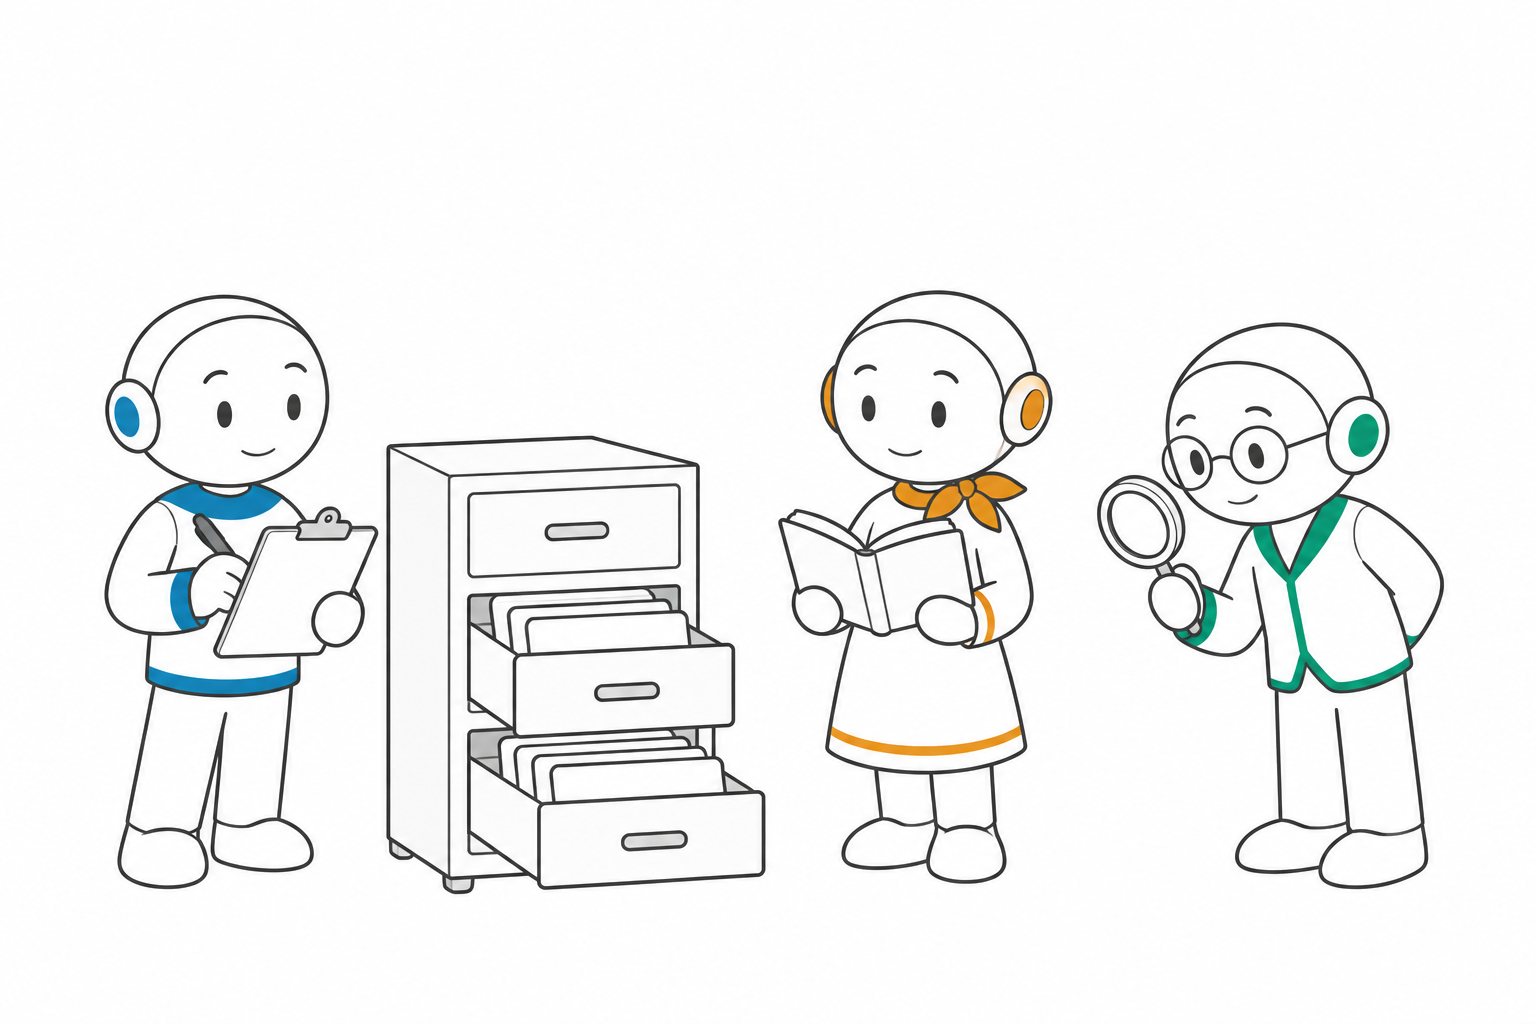
\includegraphics[width=0.46\linewidth]{../../assets/en/roles-memory-concept.png}\par
{\scriptsize Conceptual role-and-memory artwork, AI-generated; not an experimental result.}
\end{center}

\clearpage{\small\linespread{0.98}\selectfont\setlength{\parskip}{0pt}\tableofcontents}
\clearpage\pagenumbering{arabic}
\chapter{Executable Data Synthesis and Filtering}\label{ch:data}\section{Research objective and framework foundations}
Educational responses require separate checks of program facts and task completion. Giving the right output does not diagnose a learner's misconception; a plausible explanation can still give an incorrect follow-up answer. This chapter asks whether synthesized references are executable and traceable, whether filtering reduces superficial preference cues, and which limitations remain. It delivers 1,000 supervised fine-tuning (SFT) demonstrations and 500 preference pairs. Student learning is not measured.

\subsection{NaturalThoughts: which reasoning examples to retain}
NaturalThoughts generates, annotates, selects, and distils reasoning demonstrations~\cite{nat}. Questions sampled from NaturalReasoning receive DeepSeek-R1 reasoning traces and final answers. Domain labels, reasoning strategies such as verification and backtracking, and verbosity distinguish diversity from repeated narration. Selection examines topic/semantic/strategy diversity and difficulty proxies, including disagreement between models with different reasoning behavior. Disagreement does not prove either answer correct. In mixed distillation, disagreement examples retain complete reasoning and other examples can retain only final answers; the selected records supervise a student model.

Its evidence is scale-dependent. With Llama-3.1-8B-Instruct and 100,000 examples, disagreement selection versus random sampling gives 45.2\% versus 42.5\% on GPQA-Diamond; at 500,000 examples, the values are 45.2\% versus 48.3\%~\cite{nat} (p.~7, Table~1). This project borrows separate selection attributes and independent output checks. It does not reproduce DeepSeek-R1 generation, the paper's annotations, or large-model distillation. Structural difficulty labels have no student calibration.

\subsection{Matrix: how heterogeneous generation stages execute}
Matrix wraps each input in a serializable orchestrator containing workflow state, intermediate history, and routing decisions~\cite{matrix}. Queue-driven agent actors update that item and pass it to the next stage; completed items reach a persistent sink. Inference and containerized tools are separate services. Row-level scheduling and data/task/agent parallelism allow individual items to advance without waiting for a heterogeneous batch. Monitoring tracks queues, outstanding work, and latency. Its at-most-once behavior requires recording failures: restarting an actor does not automatically recover a dequeued in-flight item.

In webpage-to-reasoning synthesis, document filtering, question/reference extraction, independent solving, and optional verification are distinct stages. Scheduling does not determine answer quality; task-specific checks do. The paper reports approximately 6.8 times Coral's throughput using the same model and 248 A100 GPUs, with each system's own concurrency and similar reported consensus correctness~\cite{matrix} (p.~9, Table~1). The local implementation borrows separation of stages and per-item provenance; it deploys no distributed Matrix cluster and claims no corresponding speedup.

AIR separates preference annotation, instruction selection, and pairing~\cite{air}; fDPO filters against a current-model-dependent reward comparison~\cite{fdpo}; DEITA combines complexity, quality, and embedding diversity~\cite{deita}. These inform design choices, without importing their thresholds or claiming their model improvements. The cited papers supply the original mechanisms and their evidence boundaries.

\begin{figure}[H]\centering
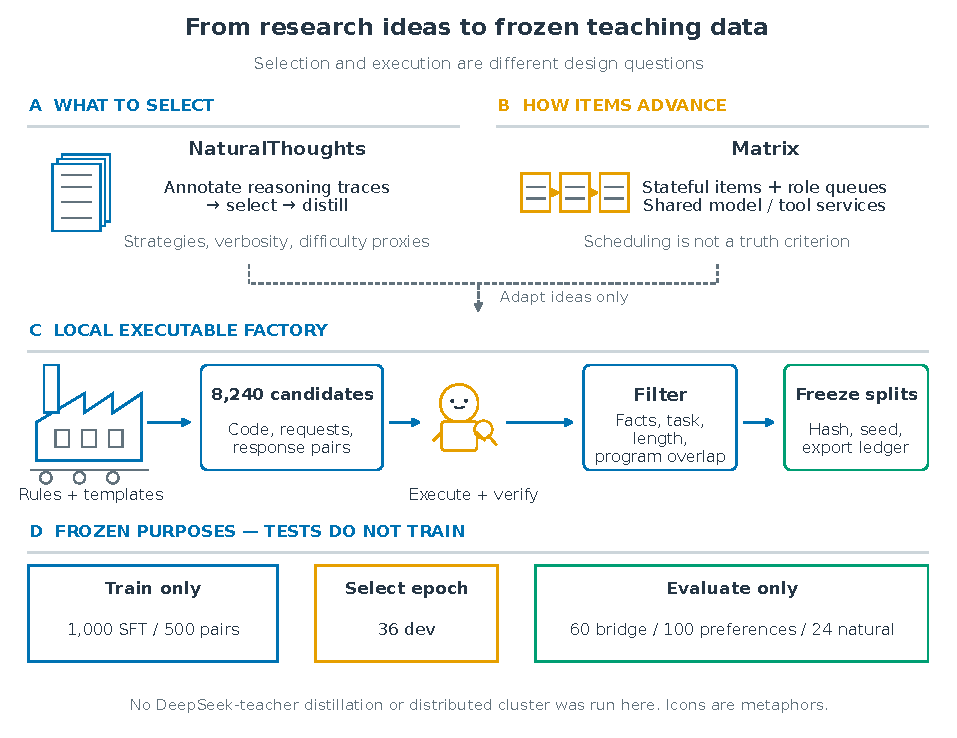
\includegraphics[width=\linewidth]{../../assets/en/synthesis-atlas.pdf}
\caption{From two research inspirations to a bounded executable dataset. The framework contributions, implemented verification, and frozen training/evaluation exports are distinct. The factory and inspector are explanatory metaphors, not additional agents or experimental subjects.}\label{fig:data-pipeline}
\end{figure}\FloatBarrier

\section{Executable data construction and verification}
An SFT record has user/assistant messages; a preference record has a shared prompt and chosen/rejected responses. Metadata binds family, task, structural difficulty, seed, candidate ID, program, reference, filtering decision, and export row. The revised generator records 8,240 candidates across 24 training families. Prediction, explanation, diagnosis, and transfer each receive 250 SFT examples. Negatives comprise 250 factual errors and 250 instruction mismatches, such as omitting an explicitly requested explanation. These rule-constructed contrasts are not naturally sampled model errors. Chinese requests and responses remain unchanged in the frozen files; English examples are translations. No online teacher model generates each row, and there are no student observations or teacher preference votes.

For original program $P$ and follow-up $P'$, independently computed outputs $y,y'$ must satisfy
\begin{equation}
V(P,P')=\mathbf1\{\operatorname{stdout}(P)=y\}\mathbf1\{\operatorname{stdout}(P')=y'\}.
\label{eq:data-exec}
\end{equation}
The auditor uses the standard library without importing the generator/renderer, checks tagged references and negative types, and requires answer-changing variants where intended. Exact normalized programs and prompts are checked across splits, including original/follow-up combinations. A coarser AST measure removes names and constants to expose template repetition; it serves a different purpose from exact deduplication. Shared project authorship still limits independence.

Exports contain 1,000 SFT demonstrations, 500 preference pairs, 36 development demonstrations from three held-out families, 60 byte-preserved earlier bridge references, 100 held-out preference pairs, and 24 separately authored natural questions. Development records select checkpoints; tests do not. Natural questions are Codex-authored within the project and some topics overlap training, so they test new instances/phrasing rather than wholly unseen knowledge. The revised audit passes 11,234 heterogeneous checks and regenerates ten principal files identically. This supports traceability and executable consistency, not an 11,234-item pedagogical pass rate.

\section{Filtering comparison and residual shortcuts}
The earlier release permits a controlled selection study on the same 1,931 eligible preference candidates. Fifty paired permutations compare random selection (A), task/background/defect balancing (B), and additional length priority (C), with fixed family quotas and 500 selected pairs each. Unshuffled C reproduces the published IDs. These are order permutations of one pool, not 50 independently collected datasets. Define
\begin{equation}
H=(n_{\mathrm{preferred\ longer}}+0.5n_{\mathrm{equal}})/N.
\label{eq:data-heuristic}
\end{equation}
The label imbalance $D$ is the family-quota-weighted mean total-variation distance $\frac12\sum_k|p_k-1/K|$ across task, background, and defect axes.

\begin{table}[H]\centering\small
\caption{Selection on one fixed pool: means (sample SD over 50 permutations); $D$ reports means only.}\label{tab:data-ablation}
\begin{tabularx}{\linewidth}{@{}Yrrr@{}}\toprule
Policy & \shortstack{Chosen shorter\\(\%)} & \shortstack{Choose-longer $H$\\(\%)} & $D$\\\midrule
A: random & 19.08 (1.43) & 80.63 (1.44) & 0.1112\\
B: labels & 19.39 (1.03) & 80.31 (1.02) & 0.0189\\
C: length + labels & 43.89 (0.12) & 55.97 (0.15) & 0.0278\\\bottomrule
\end{tabularx}
\end{table}\FloatBarrier

\begin{figure}[H]\centering
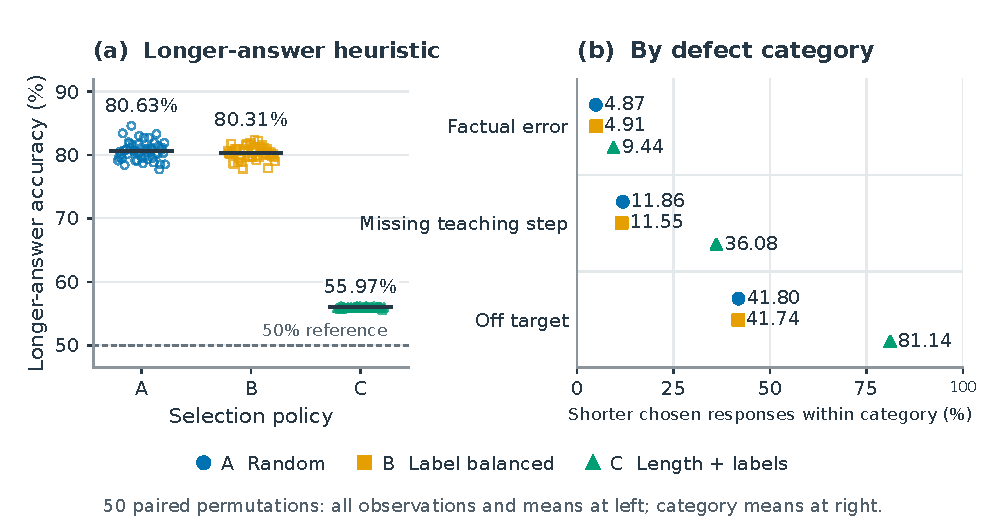
\includegraphics[width=\linewidth]{../../assets/en/selection-ablation.pdf}
\caption{Observed length cues under three selection policies. Points retain all 50 paired permutations; category means expose cues concealed by the aggregate. No model is trained for this comparison.}\label{fig:data-ablation}
\end{figure}\FloatBarrier

Adding length priority reduces $H$ relative to B in every permutation: mean $-24.34$ percentage points, SD 1.02, range $[-26.3,-21.7]$. Label imbalance increases from 0.0189 to 0.0278, documenting a trade-off. Under C, shorter-chosen proportions still differ by negative category: 9.44\% factual errors, 36.08\% teaching omissions, and 81.14\% objective shifts.

Family supply explains why nearest-half balancing does not achieve 250 shorter-chosen pairs. Floor-half targets sum to 245, while list aliasing, loop control, and recursion lack 14, 7, and 5 pairs. Seven odd-quota families can each contribute one extra. Thus the family-nearest-half feasible total is 219--226; the published set has 220 and the permutations 219--221. Overall 250 is possible only by letting some families compensate for others and depart from internal half balance.

\begin{figure}[H]\centering
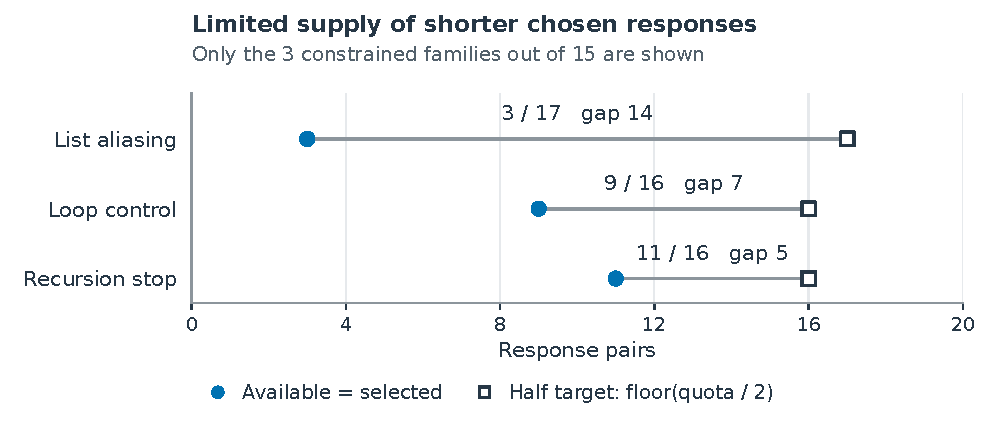
\includegraphics[width=\linewidth]{../../assets/en/family-supply.pdf}
\caption{Three of 15 original training families lack enough shorter-chosen candidates to reach floor-half quotas. All available shorter-chosen pairs in these families are selected; annotated deficits explain the remaining constraint.}\label{fig:data-family-supply}
\end{figure}\FloatBarrier

The original off-topic negatives also leak labels through three mutually exclusive literal fragments: 58 contain \verb|sep='-'|, 62 contain \verb|end=''|, and 59 contain \verb|print('A#B')|. None of the other 321 negatives or 500 chosen responses matches. The revision removes these known cues and shortens responses, but does not prove removal of all shortcuts.

\begin{table}[H]\centering\small
\caption{Published-release diagnostics under matched definitions. The 55.9\% published-set value differs from the 55.97\% permutation mean.}\label{tab:data-revision}
\begin{tabularx}{\linewidth}{@{}Yrr@{}}\toprule
Diagnostic & Earlier & Revised\\\midrule
SFT / preference AST structures & 105 / 98 & 145 / 121\\
Median SFT / chosen characters & 306 / 296 & 65 / 64\\
Choose-longer success & 55.9\% & 50.0\%\\
Negatives with checked fixed cues & 179 & 0\\\bottomrule
\end{tabularx}
\end{table}\FloatBarrier

Residual coupling remains strong: of 250 factual-error negatives, 122 are transfer and 121 diagnosis, versus six prediction and one explanation; all 250 instruction-mismatch negatives are prediction/explanation. The preference test has a related association. All 1,000 SFT answers use the same output label once, reduce to 145 structures, and contain 890 distinct complete responses; the 36 development rows contain only four structures. Executability therefore coexists with limited pedagogical and protocol coverage.

\section{Conclusion and supplementary evidence}
The data study implements generation and filtering and measures specific surface-cue changes. It does not establish improved reasoning, teacher-rated quality, or student learning. Twelve historical qualitative checks are non-blind Codex inspection, not a corpus-wide success estimate. Candidate ledgers, per-item reviews, legacy fingerprint definitions, and the complete C00670 preference example remain in the published synthesis data and comparison records. The downstream model tests the stronger reliability claim in Chapter~\ref{ch:training}.
\FloatBarrier
\chapter{Supervised Fine-Tuning and Preference Optimization}\label{ch:training}\section{Experiment question, model, and objectives}
The experiment starts from the official \texttt{Qwen/Qwen2.5-0.5B} base, then applies SFT and DPO using the filtered educational data. The pinned revision begins \texttt{e332bac62ed3}; weights, tokenizer, and configuration have recorded hashes~\cite{qwenbase}. The model has 494,032,768 parameters and 24 Transformer layers. It is not the Instruct variant; Chapter~\ref{ch:agents}'s separately sourced Instruct diagnostic is not credited to this training. The research question is whether fitting demonstrations and optimizing pairwise preference improves generated teaching, assessed through matched questions and factual review.

LoRA freezes $W_0$ and learns $(\alpha/r)BA$ in query/value projections~\cite{lora}. Shared explicit ChatML serialization adds no system turn. Complete responses include the turn terminator; prompt and padding positions are masked, and selected training examples are not silently truncated. SFT minimizes response-token-normalized NLL:
\begin{equation}
\mathcal L_{\mathrm{SFT}}=-\frac1T\sum_{t=1}^T\log\pi_\theta(y_t\mid x,y_{<t}).
\label{eq:training-sft}
\end{equation}
DPO starts both policy and frozen reference from the selected SFT checkpoint. Reference sequence scores are cached before updates. With whole-response log probability $\ell_\pi$, preferred/dispreferred answers $y^+,y^-$ share the prompt:
\begin{align}
m_\theta&=\ell_{\pi_\theta}(y^+|x)-\ell_{\pi_\theta}(y^-|x)
-\bigl[\ell_{\pi_{\rm SFT}}(y^+|x)-\ell_{\pi_{\rm SFT}}(y^-|x)\bigr],\\
\mathcal L_{\mathrm{DPO}}&=-\log\sigma(0.1m_\theta).
\label{eq:training-dpo}
\end{align}
This relative objective~\cite{dpo} is not a factual-correctness score. Equal initial policy/reference predicts loss $\ln2$, supplying one integrity check alongside parent hashes and measured weight changes.

\section{Actual computation and model selection}
The historical CPU run uses an i7-12700H, approximately 16~GB RAM, six threads, and float32. It trains 128 SFT demonstrations and 64 preference pairs once, adapting the last four layers with $r=8$, $\alpha=16$ and 90,112 parameters. Learning rates are $8\times10^{-4}$ and $2\times10^{-4}$. All 15 original training families are represented; each stage uses 12.8\% of its released data. Both stages actually change weights. Its results remain separate because later experiments change the dataset and configuration together.

\begin{table}[H]\centering\small
\caption{Historical CPU results: complete references for 60 questions (13,437 response tokens); other measures use six greedy generations with a 192-token cap. Automatic unresolved labels are not factual errors.}\label{tab:training-cpu}
\begin{tabularx}{\linewidth}{@{}Yrrrr@{}}\toprule
Stage & Reference NLL & Automatic C/W/U & At cap & Repetition (\%)\\\midrule
Base & 3.276 & 0 / 0 / 6 & 6 & 44.9\\
SFT & 2.508 & 0 / 2 / 4 & 5 & 58.0\\
DPO & 2.664 & 0 / 0 / 6 & 6 & 72.8\\\bottomrule
\end{tabularx}
\end{table}\FloatBarrier

Both genuine cloud experiments use all 1,000 revised SFT examples over three epochs, 500 DPO pairs once, and a 500-update continued-SFT control from the same selected parent. They use float32, batch one, $r=16$, $\alpha=32$, seed 20261107, and DPO coefficient 0.1. The control uses the SFT split, not the chosen responses to the same DPO prompts; it matches updates and selected settings, not prompts, token counts, or strict compute.

\begin{table}[H]\centering\small
\caption{Recorded cloud configurations and development selection. Times sum optimization steps, excluding loading, reference caching, and evaluation.}\label{tab:training-protocol}
\begin{tabularx}{\linewidth}{@{}Yrr@{}}\toprule
Setting & First cloud run & Exploratory retry\\\midrule
Adapted Q/V layers & Last 8 & All 24\\
Trainable parameters & 360,448 & 1,081,344\\
SFT learning rate & $2\times10^{-4}$ & $1\times10^{-4}$\\
DPO / control learning rate & $1\times10^{-5}$ & $1\times10^{-5}$\\
SFT / DPO / control updates & 3000 / 500 / 500 & 3000 / 500 / 500\\
Dev NLL: epoch 1 & 2.6449 & 2.8672\\
Dev NLL: epoch 2 & 3.0709 & 3.3245\\
Dev NLL: epoch 3 & 3.3794 & 3.6293\\
Step seconds: SFT / DPO / control & 251.5 / 68.9 / 44.1 & 411.9 / 103.8 / 70.9\\\bottomrule
\end{tabularx}
\end{table}\FloatBarrier

Each run processes 143,934 SFT response tokens, 48,091 two-sided DPO tokens, and 23,981 control tokens. Complete-reference NLL on 36 development examples selects epoch one at 1,000 updates in both runs, preferring earlier epochs on ties. The 3,000-update SFT budget includes unselected epochs. Development covers only four coarse structures. Retry planning follows earlier test observations and simultaneously changes layer scope and SFT learning rate, so it is exploratory and cannot isolate either factor. The first package independently records CUDA but not the device name; retry Torch and \texttt{nvidia-smi} logs record T4 in both attempt records. Device logs are not external hardware attestation. 

\section{Paired outcomes and full-text review}
The fixed evaluation uses 24 Codex-authored natural questions, 100 held-out preference pairs, and 60 byte-preserved bridge references. Development records do not enter final metrics. All stages use identical prompts, greedy decoding, and a 384-new-token cap, preserving raw text, tokens, and stop reasons. NLL is token-weighted over complete references including terminators. Preference win proportion compares complete-sequence likelihoods and is length-sensitive, not human preference or student learning. The retry reuses an observed test rather than creating a new blind assessment.

Separate Codex reviewers read complete outputs, recording hashes, continuous evidence, interpretations, and reasons. A unique discernible primary claim matching execution is correct (C); a unique different claim is wrong (W). Missing answers, copied input, unclear roles, and unretracted conflicting claims remain unresolved (U). Explanation facts are checked separately. This is same-project, non-blind model-assisted review, not external teacher assessment.

\begin{table}[H]\centering\small
\caption{Matched cloud outcomes: 24 natural questions, 60 bridge references, and 100 preference pairs. EOS counts termination; C/W/U use full-text primary-output review. Preference and repetition columns are percentages.}\label{tab:training-cloud}
\begin{tabularx}{\linewidth}{@{}Yrrccrr@{}}\toprule
Stage & \shortstack{Natural\\NLL} & \shortstack{Bridge\\NLL} & \shortstack{EOS\\/24} & C/W/U & Pref. & Repeat\\\midrule
Base & 3.7258 & 3.2758 & 7 & 3/3/18 & 43 & 63.3\\
First SFT & 3.5892 & 4.0081 & 1 & 1/20/3 & 47 & 79.2\\
First DPO & 4.2992 & 4.5216 & 1 & 0/7/17 & 51 & 76.3\\
First control & 3.4445 & 3.9352 & 0 & 1/19/4 & 47 & 82.5\\
Retry SFT & 3.5873 & 4.2234 & 8 & 3/16/5 & 45 & 55.7\\
Retry DPO & 6.6152 & 6.7619 & 11 & 4/7/13 & 53 & 31.2\\
Retry control & 3.5764 & 4.3570 & 7 & 5/11/8 & 47 & 63.0\\\bottomrule
\end{tabularx}
\end{table}\FloatBarrier

First-cloud DPO worsens reference NLL on all 24 natural and 60 bridge items relative to SFT; continued SFT improves all 84 references but still fails to deliver reliable teaching. Retry SFT reduces repetition and ends more responses, while natural NLL changes only $-0.0019$ from first SFT. Retry DPO again worsens all 84 references despite preferred-sequence wins rising from 45\% to 53\% and EOS from 8 to 11. These endpoints do not support one aggregate claim of improvement.

\begin{figure}[H]\centering
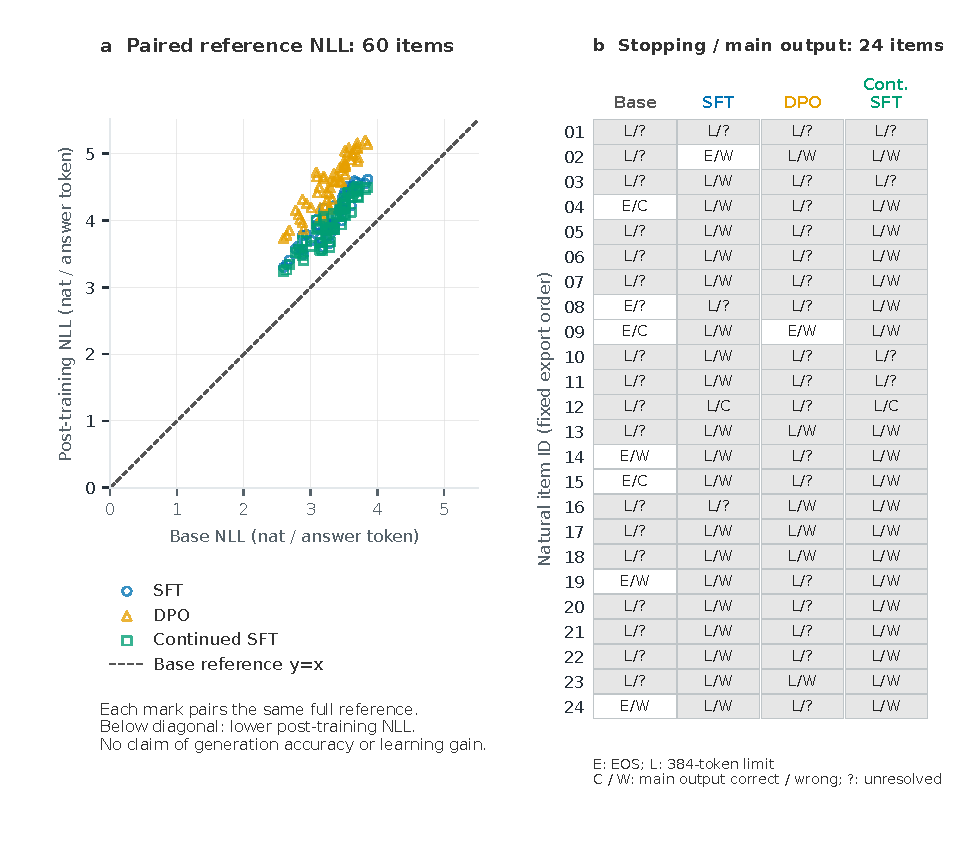
\includegraphics[width=\linewidth]{../../assets/en/training-v2-evidence.pdf}
\caption{First-cloud itemwise evidence: 60 paired bridge NLL values and 24 natural-question stopping/output records per stage. E denotes EOS, L the 384-token cap, and C/W/? full-text primary judgments; explanations are reviewed separately. All marks are recorded observations, with no seed-level significance claim.}\label{fig:training-v2-evidence}
\end{figure}\FloatBarrier

All three correct retry-SFT primary values have direct explanation errors. Of four correct retry-DPO values, three have false explanations and one is unclear. Of five correct control values, three explanations contain errors, one is unclear, and one has no identified factual error but still repeats severely. For example, SFT gives 11 for \verb|137 // 12| yet claims no remainder (the remainder is five); it gives 181 for \verb|[173,179,181,191][-2]| yet says negative indexing starts at zero. Correct values are therefore not complete teaching successes. The retry's 24 base responses exactly match the first run and reuse checked judgments; all 72 new trained responses are reviewed afresh.

\begin{figure}[H]\centering
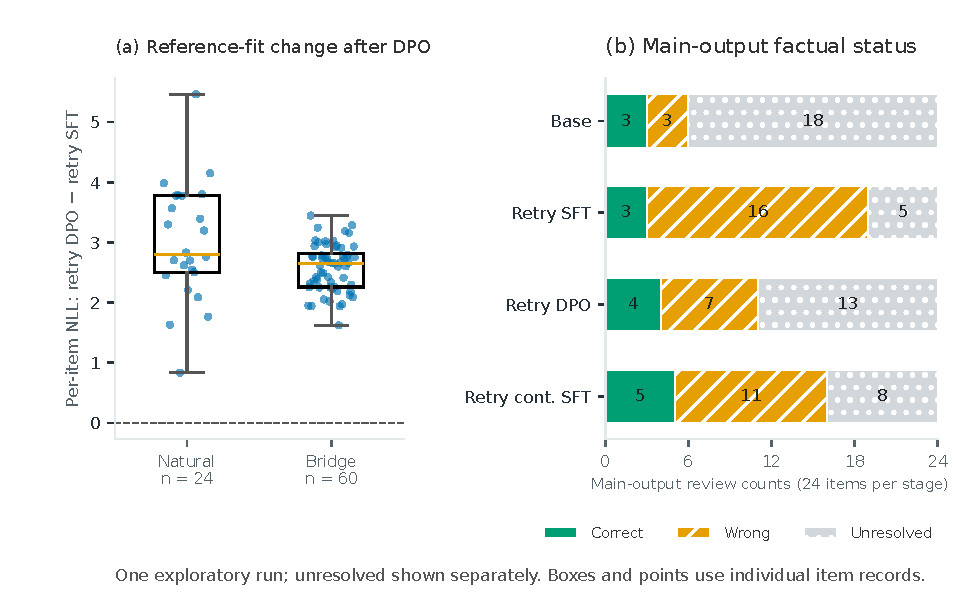
\includegraphics[width=\linewidth]{../../assets/en/training-retry-comparison.pdf}
\caption{Retry DPO-minus-SFT reference NLL and primary-output review. All 24 natural and 60 bridge items worsen in NLL; boxes summarize the recorded item distribution, not variability across training seeds. Unresolved remains distinct from wrong.}\label{fig:training-retry-comparison}
\end{figure}\FloatBarrier

\section{Two fixed questions: task, execution reference, and recorded behavior}
The following are the first two exported natural questions, fixed rather than selected for success. English excerpts translate recorded Chinese responses; ellipses mark omissions. Table judgments use the complete response, including contradictions absent from short excerpts. They are not new English generations or revised scoring rules.

\Needspace{25\baselineskip}
\subsection{NATURAL-01: assignment preserves an earlier value}
\begin{quote}\small
``I thought saved would decrease along with wallet. Can you tell me what is actually printed and explain what is wrong with that understanding?''
\begin{verbatim}
wallet = 137
saved = wallet
wallet = wallet - 18
print(saved)
\end{verbatim}
\end{quote}
Execution reference: \texttt{137}. Rebinding \texttt{wallet} does not change the integer value already bound to \texttt{saved}.

\begin{table}[H]\centering\small
\caption{Case 01: translated short excerpts and full-response primary judgments.}\label{tab:training-case01}
\begin{tabularx}{\linewidth}{@{}lYc@{}}\toprule
Stage & Recorded excerpt, translated & C/W/U\\\midrule
Base & ``It subtracts 18 from wallet and stores the result in saved.'' No unique original-program output. & U\\
First SFT & ``Output: 49'' \ldots\ ``Output: 101.'' & U\\
First DPO & ``Output: 79'' \ldots\ ``Output: 80.'' & U\\
First control & ``Output: 119'' \ldots\ ``the printed result is 117.'' & U\\
Retry SFT & ``Output: 119''; ``print(saved) outputs 119.'' & W\\
Retry DPO & ``Output 119'' \ldots\ ``Output: 18.'' & U\\
Retry control & ``Output: 119''; ``Passing wallet as an argument to -18 makes it [137].'' & W\\\bottomrule
\end{tabularx}
\end{table}\FloatBarrier

The failures concern assignment semantics rather than a missing output label alone. Repeated or competing values cannot be resolved by selecting a convenient number, including 137 copied from the prompt.

\Needspace{25\baselineskip}
\subsection{NATURAL-02: split, slice, and join}
\begin{quote}\small
``I am processing tree labels. Which names are sliced here? What text is finally joined together? Please explain directly using this example.''
\begin{verbatim}
label = 'oak|pine|elm|ash'
parts = label.split('|')
print('/'.join(parts[1:3]))
\end{verbatim}
\end{quote}
Execution reference: \texttt{pine/elm}. Indices 1 and 2 are selected; the joining separator is a slash.

\begin{table}[H]\centering\small
\caption{Case 02: code/output strings preserve original spelling; prose is translated.}\label{tab:training-case02}
\begin{tabularx}{\linewidth}{@{}lYc@{}}\toprule
Stage & Recorded excerpt, translated & C/W/U\\\midrule
Base & Repeats the full question and code, followed by ``erable''; no result is asserted. & U\\
First SFT & ``Output: /oak|pine|elm|ash''; the slice is said to retain oak and pine. & W\\
First DPO & ``Output: /amel|ash|elm|ash'' \ldots\ repeated \texttt{|ash}. & W\\
First control & ``Output: /oak|pine|elm|ash.'' & W\\
Retry SFT & ``Output: oak|elm''; ``keep only the first and third components.'' & W\\
Retry DPO & ``Output: oak|elm'' \ldots\ ``Output: ['oak', 'oak', 'elm', 'elm', 'elm'].'' & U\\
Retry control & ``Output: oak|elm''; ``remove the first and third semicolons.'' & W\\\bottomrule
\end{tabularx}
\end{table}\FloatBarrier

The original programs, complete requests, all seven stage outputs, stop reasons, and per-item reviews remain in \path{training/retry_imports/retry_048f9a92c0ef_numeric_review/comparison/} and the linked JSONs. Thus compact excerpts do not replace or silently discard negative evidence.

\section{Integrity exception, degradation, and the stopping decision}
The first cloud import passes 552 consistency checks. The initial retry import runs 965 checks and fails one first-step policy/reference threshold. Rejected-sequence scores differ by $1.52587890625\times10^{-5}$, one float32 representable step at that magnitude, whereas the old absolute threshold is $10^{-5}$; loss differs from $\ln2$ by $7.77\times10^{-7}$. The original failed audit is retained. A documented post-hoc review permits at most one step per sequence and checks ratios, margins, DPO scaling/loss arithmetic, and exact frozen-cache agreement. All 966 revised checks pass; boundary tests still reject larger or inconsistent discrepancies. A CPU probe does not reproduce the T4 reduction cause. This changes neither weights, outputs, nor factual labels and establishes internal consistency rather than effectiveness.

Inspection finds no obvious prompt-mask reversal, causal-shift error, omitted terminator, or truncation loss of the terminator. Development NLL worsens after epoch one. DPO saves only its final 500-step checkpoint, without intermediate development stopping; early stopping cannot be claimed retrospectively. Across the retry's steps 401--500, 96 of 100 pre-update training-pair snapshots score both responses below the frozen SFT reference; mean policy-minus-reference scores are $-37.761/-59.936$ nats. First-run values are 84 snapshots and $-8.550/-13.065$. Each snapshot concerns that step's pair, not a before/after measurement of one update or a fixed-set endpoint curve. These records show a larger relative preference margin alongside lower absolute likelihood; they do not isolate the cause of degraded generation. 

\paragraph{Observed limitations and possible causes.} The 1,000 SFT examples contain 145 coarse program structures; preference rejection reasons are coupled to task types, and the 36-item development set covers only four structures. Development NLL worsens after the first epoch, and the retry DPO reference NLL rises from 3.5873 to 6.6152 on the 24 natural questions. These observations indicate limited coverage and degraded reference fit, not their causes.

The small base model's capacity, narrow templates, preference shortcuts, and training choices could each contribute. No larger base was tested under the same protocol; the retry changes both layer scope and learning rate, and the continued-SFT control differs in prompts and token budget. Thus neither model size nor a single design choice can be assigned a causal share; overfitting remains a hypothesis. No additional training or model inference was performed.

\begin{figure}[H]\centering
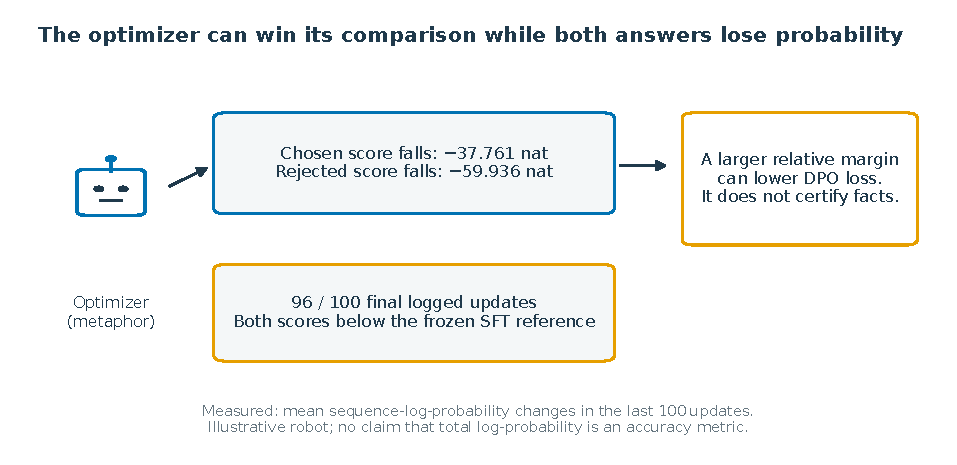
\includegraphics[width=\linewidth]{../../assets/en/training-objective-gap.pdf}
\caption{A relative preference objective can improve while both response probabilities fall. Values are pre-update, current-pair scores at steps 401--500 relative to frozen SFT, not changes caused by individual updates. The robot is a metaphor; sequence log probability is not accuracy or learning gain.}\label{fig:training-objective-gap}
\end{figure}\FloatBarrier

A single bounded local remedy, planned before its inference, mixes effective adapter updates rather than separately interpolating low-rank factors:
\begin{equation}
\Delta W_\lambda=(1-\lambda)\Delta W_{\mathrm{SFT}}+\lambda\Delta W_{\mathrm{DPO}}.
\end{equation}
No optimizer update occurs. All 36 development references select among fixed coefficients, preferring a smaller one for differences below $10^{-6}$.

\begin{table}[H]\centering\small
\caption{Bounded mixing on the development set. Zero is the SFT parent; one is complete DPO. This is post-hoc calibration, not a new blind training result.}\label{tab:training-remedy}
\begin{tabular}{@{}lrrrrr@{}}\toprule
$\lambda$ & 0 & 0.05 & 0.10 & 0.25 & 1\\
Development NLL & 2.8672 & 2.9447 & 3.0290 & 3.3237 & 5.9292\\\bottomrule
\end{tabular}
\end{table}\FloatBarrier

Zero wins, withdrawing DPO's increment within this family without repairing SFT. Six prespecified development cases then compare repetition penalties 1.0/1.08 with the same greedy 192-token cap. EOS improves from 1/6 to 3/6 and tokens fall from 970 to 717; each setting still has 0 correct, 4 wrong, and 2 unresolved primary outputs. Both report three \texttt{b}s where \texttt{aabbbbbab} has six; a loop with reference 112 receives 125 or 248. Competing Boolean claims remain unresolved. The development set is reused and has only four structures, so this is no independent validation.

The prespecified factual-failure stopping rule is met. The study ends at the recorded stopping decision: no further cloud training, test-set parameter search, or new deployment is performed. Broader data, cross-balanced preference reasons, intermediate checkpoints, and supervised anchoring remain unexecuted proposals. Complete answers, logs, numerical audits, and bounded-remedy results remain under \path{training/}. The result is a functioning SFT--DPO pipeline with poor teaching reliability, not a successful educational model.
\FloatBarrier
\chapter{Verifiable Tutoring Agents and Learner Memory}\label{ch:agents}\section{Research questions and OpenMAIC mechanisms}
This chapter tests whether explicit roles, executable evidence, and persistent learner records can turn a weak educational language model into a verifiable tutoring workflow. The evaluation separates the complete system from its model: successful retrieval or a correct fallback is not evidence of autonomous model teaching. The questions concern orchestration, use of learner evidence across turns, and the mechanisms behind successful and failed teaching requests.

The source analysis uses official OpenMAIC commit \texttt{5bd8cc840ee63}, retrieved on 6 November 2026~\cite{openmaic}. The full identifier, permanent links, and SHA-256 checksums of 19 archived files are in \path{tutor/legacy/research/source_manifest.json}. OpenMAIC itself was not deployed; the Python implementation is an independent simplification. Four mechanisms inform the design:

\begin{table}[htbp]\centering\small
\caption{OpenMAIC mechanisms and pinned source anchors. Paths are relative to the pinned upstream repository; permanent links remain in the source manifest.}\label{tab:concise-agents-source}
\begin{tabularx}{\linewidth}{@{}p{25mm}Yp{65mm}@{}}\toprule
Mechanism & What the source actually implements & Source anchors\\\midrule
Roles and scheduling & Teacher, assistant, and classmates have different prompts/actions. A Director selects speakers with \texttt{call\_agent}; useful roles, not fixed round-robin turns, are requested. Child roles can share one model object. Ending actions check that a visible/substantive response exists. & \path{registry/built-in.ts}:12--155; \path{pi/director-loop.ts}:95--221; \path{pi/tools/call-agent.ts}:735--757, 847--864.\\
Course state and evidence & Material analysis/research precede outline and scene generation. Completed steps are explicit state. \texttt{read\_scene} supplies page evidence to subsequent role calls, limiting unsupported guessing. & \path{generation/run/plan.ts}:45--103; \path{generation/src/scene-builder.ts}:21--116; \path{pi/tools/read-scene.ts}:97--124.\\
Context and memory & Child history retains 12 messages. Director compaction preserves goals and unresolved work. PBL Instructor compresses history above 30 messages toward the latest 16, extracts learner clues, and reloads \texttt{earlierSummary}; 4500 characters is its summary-compression threshold. & \path{pi/prompts.ts}:558--589; \path{pi/director-compaction.ts}:95--101, 136--217; \path{v2/agents/instructor-memory.ts}:22--138.\\
Feedback and fallback & Quiz state differs before/after submission. Submitted answers, references, scores, and comments guide feedback. Unparseable model grading can fall back to half credit, which preserves interface operation rather than proving answer correctness. & \path{summarizers/state-context.ts}:172--240; \path{api/quiz-grade/route.ts}:56--105.\\\bottomrule
\end{tabularx}
\end{table}\FloatBarrier

OpenMAIC therefore has more than chat history: it includes scene state and explicit learner-summary mechanisms. However, keyword-derived progress clues are not verified mastery measurements. The project retains role separation, shared evidence, and explicit control while replacing broad multimedia classroom interaction with executable Python-output tasks. It does not reproduce speech, whiteboards, or a complete course editor.

\section{Implementation and verifiable learner memory}
The controller sequentially calls a planner, teacher, and reviewer. Roles share one loaded model, initially the Chapter 2 SFT adapter; later deployments use genuine cloud SFT checkpoints or a separately identified official Instruct model. No weights are updated in this chapter. Planning proposes focus/strategy; teaching returns answer, feedback, explanation, and optional \texttt{followup\_code}; review returns \texttt{approved} and a reason. Actual prompts are Chinese. Complete templates and every executed context, raw response, token identifier, stop reason, and adoption decision remain in the evidence files.

A bounded AST interpreter computes program output and traces. Generated text is not passed to unrestricted \texttt{eval}/\texttt{exec}. The evaluator separately executes reviewed, frozen references in CPython; unsupported programs cannot inherit a reference answer as if verified. Original adoption checks cover the answer, required explanation/feedback text, reviewer approval, and executable follow-ups. Revised controllers add explicit student-status, factual-evidence, and requested code-modification contracts; these stronger checks were absent from the historical C08 run. These gates do not prove all natural-language explanations. Rejected drafts are preserved, and the final response explicitly identifies tool/template fallback.

Original CPU inference uses float32, six threads, greedy decoding, 256 new tokens per role, and a 4096-token input-plus-generation boundary that raises an error rather than silently truncating history. Revised role budgets are 64/192/96. The implementation, model, prompts, and budget of each run are separately frozen.

\begin{figure}[htbp]\centering
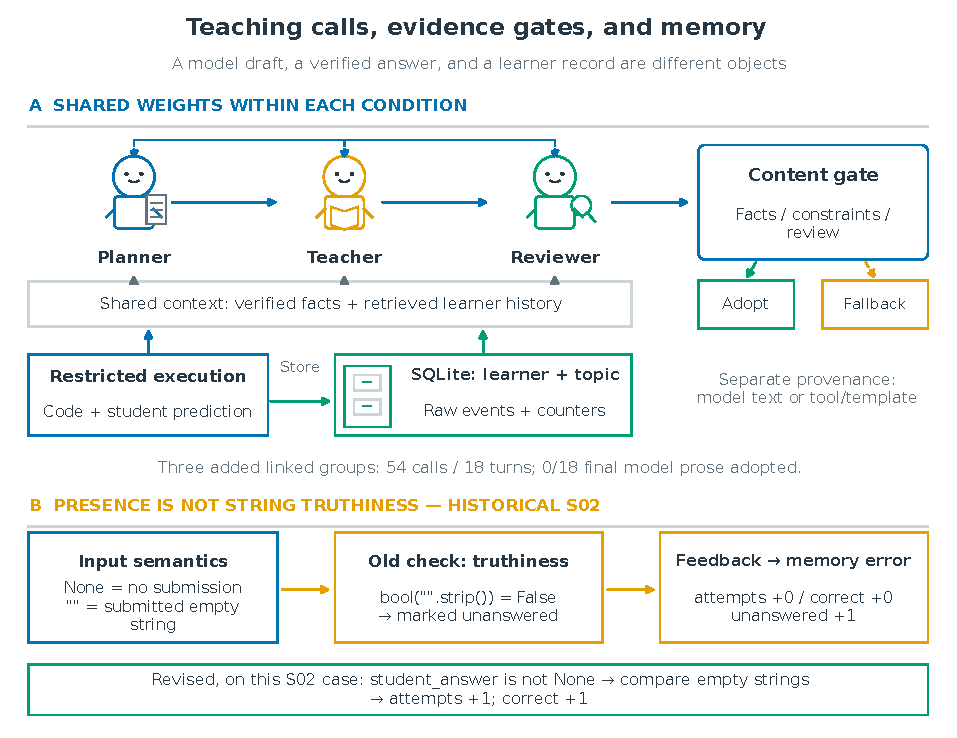
\includegraphics[width=\linewidth]{../../assets/en/teaching-memory.pdf}
\caption{Shared model, role-specific calls, independent evidence checks, and learner memory. The historical empty-string bug is distinguished from its subsequent repair. Friendly role icons explain responsibilities; they are not independently trained models.}\label{fig:concise-agents-system}
\end{figure}\FloatBarrier

SQLite stores raw episodes and derived counters. Episodes retain learner identifier, topic, program, prediction, evidence, role outputs, and final response. Counters distinguish interactions, submitted attempts, correct, incorrect, unanswered, and unverified events. A transaction writes both layers; duplicate event identifiers cannot increment counts twice. Model answers are never counted as student attempts. For learner $u$, topic $k$, and structural difficulty $d$, let $v_t$ indicate verified execution, $a_t$ submitted prediction, and $z_t$ agreement with verified output:
\begin{equation}
N_{u,k,d}\leftarrow N_{u,k,d}+v_ta_t,\qquad
C_{u,k,d}\leftarrow C_{u,k,d}+v_ta_tz_t.
\end{equation}
These are descriptive counts, not calibrated mastery probabilities. The historical approximation of $a_t$ by nonempty text is tested in S02 below.

Retrieval matches the caller-supplied learner ID and topic and supplies the latest three episodes. This assumes a trusted caller; ID filtering is not authentication. Reconstructing the system object reads the same database. Difficulty advice examines recent verified predictions at the same structural difficulty among the latest 100 relevant events, explicitly including the current answer: three consecutive correct predictions suggest an increase; two incorrect suggest a decrease; otherwise it holds. Actual exercise difficulty is checked separately. Exact topic keys, restricted syntax, and uncalibrated thresholds limit personalization; synonym resolution, prerequisites, and forgetting are unimplemented.

\section{Historical protocol and four complete case studies}
The core batch freezes eight scenarios/11 turns; after observing it, a supplementary batch freezes four scenarios/six turns. References include 22 core and 12 supplementary programs/follow-ups executed independently. Complete success requires every necessary automatic check and every predeclared qualitative item to pass. Codex technical review retains textual evidence; it is not blinded teacher assessment. Supplementary design deliberately extends coverage, with implementation hidden from its designer but original cases/results available. It is neither a random sample nor an entirely external blind test.

Together, 12 scenarios produce seven complete and five incomplete tasks, 145/150 automatic checks, and 51 real role calls. No role response is adopted; all 17 final responses use tools/templates. C03/C04 exceed frozen partial-completion expectations. C08/S02 fall below their respective frozen full-completion expectations. C07 remains an expected limitation and is not relabelled. The frozen C03 rationale mentioned earlier ``range/pairing'' errors, but the training study did not actually test range generation; this is retained as a cross-concept risk conjecture, not an observed prior range failure.

\begin{figure}[htbp]\centering
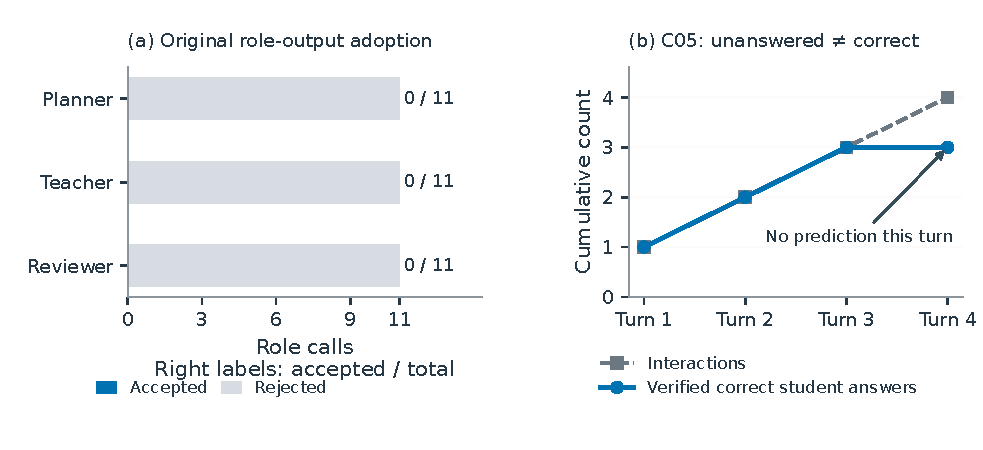
\includegraphics[width=\linewidth]{../../assets/en/agents-evidence.pdf}
\caption{Historical observations: zero accepted role outputs across 11 core turns; in C05, a fourth interaction without a prediction does not increase the three correct attempts. Automatic bookkeeping and pedagogical completeness are different criteria.}\label{fig:concise-agents-evidence}
\end{figure}\FloatBarrier

All quoted responses below are \emph{English translations of recorded Chinese excerpts}, not new English model generations. Complete tasks, references, raw role outputs, final responses, and hashes remain in \path{tutor/legacy/results/core/}, \path{tutor/legacy/results/supplement/}, and \path{reports/case-study-evidence.en.json}.

\Needspace{18\baselineskip}
\subsection{C03: retrieving an earlier mistake across instances}
\paragraph{Task and reference.}
The learner previously included endpoint 8 in \texttt{range(2,8,2)}, predicting 20 rather than 12. After reconstructing the system object, the learner predicts 9, asks for feedback linked to the old mistake, and requests a supplied same-concept follow-up:
\begin{verbatim}
total = 0
for n in range(3, 9, 3):
    total += n
print(total)
\end{verbatim}
The correct result is $3+6=9$, excluding endpoint 9. Changing the endpoint to 12 in the supplied follow-up gives $3+6+9=18$.

\Needspace{12\baselineskip}
\paragraph{Actual response and interpretation.}
The raw teacher repeats instructions about checking misconceptions, fails the structured contract, and is rejected. The final response includes:
\begin{quote}\small
Your previous prediction on this concept was \texttt{'20'}; the verified output was \texttt{'12'}. Your words were ``I included 8 as well, so I guessed 20.'' This is answer evidence, not a mastery conclusion.

Output: 9. Your current prediction agrees with execution. \texttt{range(3,9,3)} takes \texttt{[3,6]}; endpoint 9 is excluded. Follow-up reference output: 18.
\end{quote}
Two predictions remain in the database, one correct and one incorrect. This exceeds the partial expectation because retrieval survives object reconstruction and preserves old evidence. The quote comes from deterministic database access and the explanation from execution traces, not demonstrated model reasoning about learner history.

\Needspace{17\baselineskip}
\subsection{C04: separating a new learner on the same topic}
\paragraph{Task and reference.}
A different learner provides no prediction, requests explanation and the supplied follow-up, and must not inherit the previous learner's history:
\begin{verbatim}
total = 0
for n in range(2, 8, 2):
    total += n
print(total)
\end{verbatim}
The original result is $2+4+6=12$. The supplied follow-up changes the endpoint to 10, giving $2+4+6+8=20$. Submitted and correct counts should remain zero.

\Needspace{10\baselineskip}
\paragraph{Actual response and interpretation.}
The raw teacher repeatedly lists execution-step and follow-up instructions without a usable response. Final tool/template feedback states:
\begin{quote}\small
Output: 12. No prediction was provided, so this is not recorded as a correct or incorrect answer. \texttt{range(2,8,2)} takes \texttt{[2,4,6]}; endpoint 8 is excluded. Follow-up reference output: 20.
\end{quote}
Retrieval is empty. After writing, the new learner has one interaction, zero attempts, and one unanswered event. No old student's misconception is cited. This exceeds the partial expectation and verifies identity-scoped retrieval for this input, not deep adaptation to different learning backgrounds.

\Needspace{21\baselineskip}
\subsection{C08: correct execution but an invalid constrained follow-up}
\paragraph{Task and reference.}
The learner predicts 230 and asks for paired contributions, the unpaired element, and a follow-up created \emph{only by appending one number to the right list}. The task program and actually delivered follow-up are shown together:
\par\noindent\begin{minipage}[t]{0.48\linewidth}\small
\textbf{Task program}\par
\begin{verbatim}
left = [9,24,17,32,6,18]
right = [7,16,35,22,44]
total = 0
for a, b in zip(left, right):
    total += a + b
print(total)
\end{verbatim}
\end{minipage}\hfill
\begin{minipage}[t]{0.48\linewidth}\small
\textbf{Actual delivered follow-up}\par
\begin{verbatim}
left = [9,24,17,32,6,18]
right = [7,16,35,22,44]
total = 1
for a, b in zip(left, right):
    total += a + b
print(total)
\end{verbatim}
\end{minipage}\par
Five pairs contribute $16,40,52,54,50$, totaling 212; left-tail 18 is unpaired. Appending 6 to the right list is one valid reference, yielding $212+18+6=236$. Other appended values are valid when the program and explanation agree.

\Needspace{9\baselineskip}
\paragraph{Actual response and root cause.}
The unstructured raw teacher response is rejected. The final response correctly gives 212 and its pair contributions, but then says:
\begin{quote}\small
Follow-up: change only the 0 on original line 3 to 1; leave everything else unchanged. Follow-up reference output: 213.
\end{quote}
The delivered code really outputs 213 but changes the accumulator rather than the right list; it still has five pairs. All five original automatic checks pass. The missing contract is whether the edit satisfies the teaching request, not executability. This is below the frozen full expectation and is the original batch's genuine unexpected failure.

\Needspace{20\baselineskip}
\subsection{S02: a correct empty-string prediction becomes unanswered}
\paragraph{Task and reference.}
The learner explicitly submits \texttt{student\_answer=""} and says ``my prediction is an empty string, meaning one printed blank line.'' The original and supplied follow-up are
\begin{verbatim}
word = 'python'
print(word[4:1])   # Original
word = 'python'
print(word[1:4])   # Supplied follow-up
\end{verbatim}
The default positive step selects no indices in \texttt{[4:1]}. CPython emits exactly one newline; normalization leaves an empty string, matching the prediction. Attempts and correct answers should each increase once, with unanswered unchanged. The follow-up reference is \texttt{yth}.

\Needspace{12\baselineskip}
\paragraph{S02 recorded response and root cause.}
The raw teacher wrongly claims the original slice returns \texttt{python} and is rejected. The final response instead begins with a genuinely blank output field:
\begin{quote}\small
Output:

No prediction was provided, so this is not recorded as correct or incorrect. \texttt{word[4:1]} selects indices \texttt{[]} and gives \texttt{''}. Follow-up reference output: \texttt{yth}.
\end{quote}
Nothing follows the first colon in the recorded field. The interpreter and follow-up are correct, but feedback and SQLite label the submitted prediction \texttt{unanswered}; attempts/correct remain zero and unanswered increases once. Only 5/9 checks pass. The condition \texttt{bool(student\_answer.strip())} conflates valid empty content with no submission before comparing answers. This distinct state-representation failure falls below its supplementary batch's frozen full expectation, providing the second unexpected failure without changing C07's label.

\begin{figure}[htbp]\centering
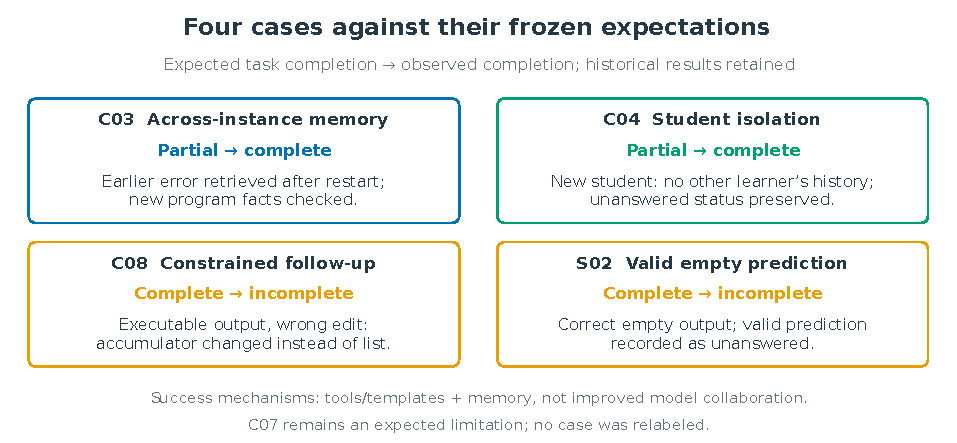
\includegraphics[width=\linewidth]{../../assets/en/case-outcomes.pdf}
\caption{Four historical cases against their own pre-run expectations. C03/C04 successes rely on verified records and templates; C08/S02 reveal different controller defects. Later repairs do not erase original outcomes or convert them into new successes.}\label{fig:concise-agents-cases}
\end{figure}\FloatBarrier

\section{Repairs, controls, and model-linkage results}
Repairs are isolated under \path{tutor/core/}; original inputs, databases, files, expectations, and labels remain unchanged. Known-case regression is not an unseen test. Fourteen unit tests additionally cover negation, edit scope, output whitespace, erroneous states, and learner separation; scripted backends are unit-test-only.

C07's missing exercise arose from a 12-character request window facing a 16-character gap. The revised detector removes that window and checks negation; bounded empty-list/dictionary default repairs use \texttt{None} and entry-time allocation. C08 now requires that removing the newly appended right-list element recover the original AST. Appending 1 yields 231, a legitimate alternative to the 236 reference. S02 distinguishes \texttt{None} from submitted empty text and removes only one trailing newline. Corrected counts are attempts +1, correct +1, unanswered +0. The first repaired tool card wrongly treats the default-expression list \texttt{[None]} as a mutable default, although the actual parameter default is \texttt{None}; the later common pipeline checks default type and entry AST and corrects that explanation. Correct code alone did not validate its teaching text.

\begin{table}[htbp]\centering\small
\caption{Controller and memory controls. Adopted text is not a teaching-quality score.}\label{tab:concise-agents-controls}
\begin{tabularx}{\linewidth}{@{}Yrrrr@{}}\toprule
Configuration & Turns & Calls & Final adoption & Checks\\\midrule
Tools/templates, memory on &17&0&0&209/209\\
Same system, memory reading off &17&0&0&204/209\\
Official Instruct, multi-role &17&51&1&209/209\\
Official Instruct, single-role subset &6&6&1&70/70\\\bottomrule
\end{tabularx}
\end{table}\FloatBarrier

The memory control still writes audit events but loses three retrieval checks (C03/S03/S04) and C05's difficulty advice/delivery checks. This supports those mechanisms, not model memory reasoning or learning gains. The external official Instruct checkpoint is not a substitute for the project's trained SFT. Thirteen of 17 raw teachers copy a numeric prompt example; all 17 reviewers approve even faulty drafts. Only C03 passes outer gates, by repeating the supplied F1 tool card verbatim. On the same six cases, single-/multi-role teacher and final texts are identical; calls are 6 versus 18 and generation times approximately 35.0 versus 73.5 seconds, without an observed final-response gain.

\begin{table}[htbp]\centering\small
\caption{Prompt/evidence diagnostics on the same eight new, prospectively frozen challenges. Tasks were informed by earlier faults. Fence compatibility was added after seeing same-task outputs and is exploratory.}\label{tab:concise-agents-prompt}
\begin{tabularx}{\linewidth}{@{}Yrrrr@{}}\toprule
Condition & Calls & Teacher parsed & Final adoption & Checks\\\midrule
No examples, free explanation &24&8/8&1/8&64/64\\
No examples, bare-JSON strict quotation &24&0/8&0/8&64/64\\
Complete-fence compatibility retest &24&8/8&1/8 quote&64/64\\\bottomrule
\end{tabularx}
\end{table}\FloatBarrier

Free explanation matches 7/8 answer fields but only 2/8 student states; its sole adoption is generic tool commentary. The strict condition's fenced raw texts manually match 7/8 answers and 3/8 states, but formal bare-JSON parsing remains zero. Complete-fence compatibility restores parsing without fixing these states; seven reviewer approvals still conflict with content requirements. Only P03 adopts \emph{model-selected tool evidence}, not independent free explanation. Raw teacher outputs are identical to the preceding strict condition; reviewer inputs change after parsing, so this is a real pipeline rerun, not offline parsing counted as new model reasoning. Exploratory pairing on the old six tasks uses 18 calls per prompt condition: free explanation adopts 2/6 but one overclaims understanding from a single correct prediction; strict quotation parses/adopts zero. Both pass 70/70 through verification and fallback. Prompt, controller, and tool-card changes occur together and are not a prompt-only ablation.

\begin{figure}[htbp]\centering
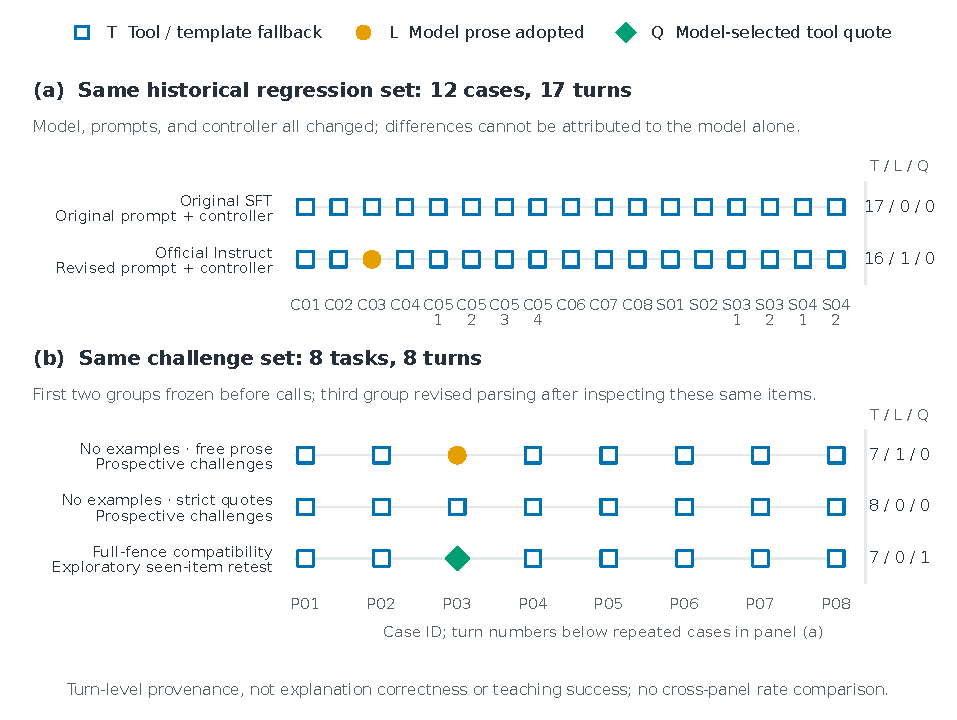
\includegraphics[width=\linewidth]{../../assets/en/agents-revision-provenance.pdf}
\caption{Recorded final-content sources: template/tool fallback, adopted model prose, and model-selected tool quotation. Panels use different task sets; no cross-panel adoption-rate comparison is valid. A selected quotation does not establish independent reasoning or teaching value.}\label{fig:concise-agents-provenance}
\end{figure}\FloatBarrier

Genuine cloud checkpoints are linked separately. The first SFT comes from the first cloud run; additional SFT comes from the exploratory retry, both indexed under \path{training/}. All conditions use the same known six cases, 64/192/96 budgets, CPU float32, and greedy decoding. No DPO weight is loaded in these linkage runs. Instruct's official serialization adds a 21-token system prefix absent from SFT. History identifiers, planner adoption, and drafts can change downstream context, preventing a weight-only causal comparison.

\begin{table}[htbp]\centering\small
\caption{Four self-trained SFT deployments on the same six cases. Each makes 18 real calls and passes 70/70 engineering checks. Normal ending means an end marker, not a correct response.}\label{tab:concise-agents-sft}
\begin{tabularx}{\linewidth}{@{}Yrrr@{}}\toprule
Pipeline/checkpoint & Tokens & Normal endings & Final adoption\\\midrule
Original repaired pipeline, first SFT &2112&0/18&0/6\\
Same pipeline, additional SFT &1914&3/18&0/6\\
Common no-example pipeline, first SFT &2112&0/18&0/6\\
Same common pipeline, additional SFT &1895&2/18&0/6\\\bottomrule
\end{tabularx}
\end{table}\FloatBarrier

The first cloud-SFT deployment adopts no role output (0/18) and no final explanation (0/6). The three added conditions contribute 54 actual calls and 5921 tokens. Within each pipeline, all six final responses are byte-identical across first/additional checkpoints and use templates. Raw text still gives wrong answers, states, and explanations: range can include an excluded endpoint while claiming exclusion; empty output becomes 9; a correct program answer can coexist with approval of a wrong student prediction. Zero adoption is therefore not merely strict formatting. The common pipeline's corrected \texttt{None} description comes from a tool-card repair, not improved model capability. Hash-bound non-blinded technical reviews remain separate from frozen runtime \texttt{unreviewed} flags.

\section{Interpretation and evidence access}
A later rendering review found that withholding answers also hid an explicitly requested exercise. The isolated fix in \path{tutor/rendering/} separates exercise delivery from answer disclosure. Six tool-only regression tests pass without model calls; historical cases, labels, and adoption rates are unchanged.

Persistent records, learner isolation, and deterministic constraints work on these inputs, but autonomous teaching, multi-role superiority, and student learning gains are unestablished. Original cases were co-developed with the system; later challenges and regressions were informed by observed faults. No same-pipeline base-model control or real-student trial supports a causal training or learning claim. Experimentation has stopped, retaining successes and genuine failures.

Full per-case scores, raw text, token/time records, all prompt variants, source hashes, and repair reviews are supplementary evidence under \path{tutor/legacy/}, \path{tutor/core/}, \path{tutor/structured/}, and \path{tutor/fence/}. These records preserve each condition without replacing its outcomes.
\FloatBarrier
\chapter{Application, Competition, and Commercial Feasibility}\label{ch:business}\section{Application objective and evidence basis}
The proposed application is supervised feedback for introductory university Python courses. Learners need diagnosis and an independently completed follow-up; teachers need control over hints, error review, and workload; departments buy and integrate the service. These are separate user, adopter, and buyer decisions. Existing assets are executable task families, trained-model baselines, program verification, and topic-scoped memory. Teacher dashboards, institutional permissions, LMS integration, correction/deletion workflows, and production monitoring remain undeveloped.

Following the business-plan guide~\cite{businesscambridge}, this chapter links use case, competition, operations, finance, and validation. Sources were checked through 7 November 2026, prioritizing original research, official statistics, and supplier documentation. Product directories inform product formats, not revenue evidence. The three evidence classes remain distinct: the data, training, and agent studies measure prototype behavior; external studies and websites describe other systems; pricing, demand, workload, conversion, and collection are commercial assumptions. No customer interview, logged-in competitor benchmark, paid teaching API trial, school purchase, or real-student pilot was conducted.

The workflow would import teacher-approved questions/tests/hint limits, require a student's own prediction or code, verify facts, supply staged feedback, route exceptions to teachers, write correctable answer evidence, and select a related follow-up. It initially supports only the declared Python subset and does not automatically grade high-stakes examinations. Original the agent study's seven complete cases out of 12 depend on tools/templates, not adopted model teaching; subsequent engineering repairs and SFT deployments do not establish institutional readiness.

\begin{figure}[htbp]\centering
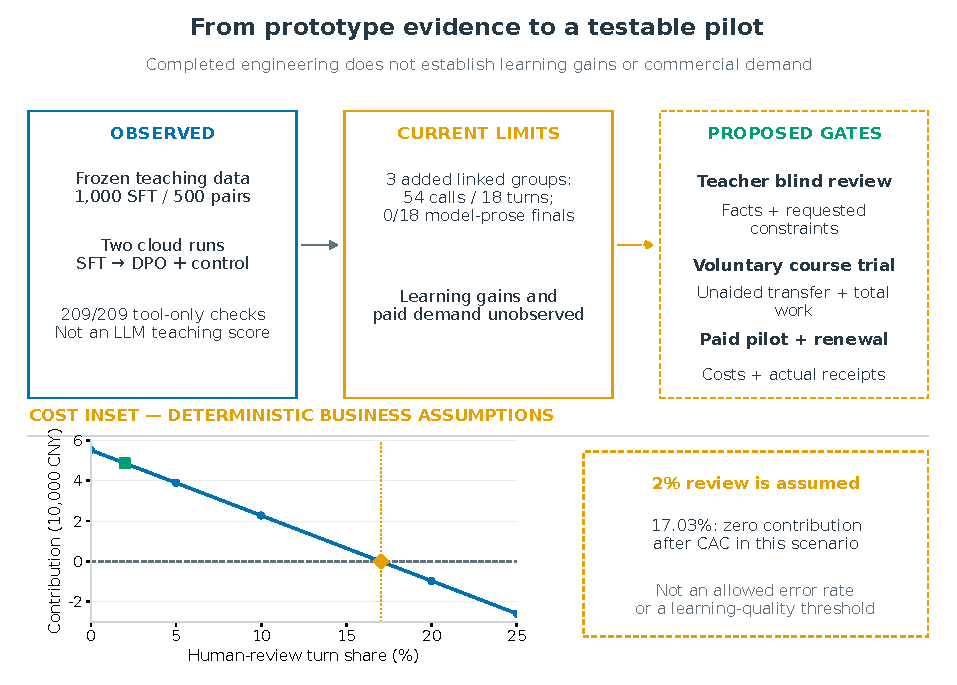
\includegraphics[width=\linewidth]{../../assets/en/evidence-to-pilot.pdf}
\caption{From research evidence to a proposed supervised pilot. Observed prototype results, external supplier claims, and business assumptions have different evidential roles. The assumed 2\% review rate and 17.03\% cost boundary are not measured quality or customer outcomes.}\label{fig:concise-business-evidence}
\end{figure}\FloatBarrier

\subsection{What external research does and does not establish}
The Ministry of Education reports 3167 higher-education institutions and 48.7257 million enrolments in 2025, across education forms~\cite{businessmoe}. Without a verified target-department list, Python enrolments, budgets, or procurement intentions, these are background rather than a validated market estimate.

Kestin et al.'s two-week, two-lesson physics crossover includes 194 of 233 enrolled students and finds benefits of an expert-designed AI tutor on immediate post-tests~\cite{businesskestin}; this system-specific result is not the project's effect. Bastani et al.'s mathematics experiment with nearly 1000 students at one Turkish high school finds approximately 17\% lower unaided exam performance for unguarded GPT Base relative to controls---a relative change, not percentage points. The guarded GPT Tutor does not demonstrate a significant positive gain on that corresponding exam outcome~\cite{businessbastani}. CodeAid's 12-week deployment in a 700-student programming course, with roughly 8000 interactions, emphasizes cognitive engagement and avoiding direct answer writing~\cite{businesscodeaid}. Together these studies motivate a pilot that separately measures assisted practice, unaided transfer, delayed retention, and teacher work; they cannot be pooled into a product ranking or a claim of demand.

\section{Competitors and differentiation hypothesis}
CodeGrade is a direct comparator for programming assignments, tests, feedback, and teacher workflow. Khanmigo is a broader tutoring and institutional-procurement comparator. Their selection reflects task relevance, not market-share rank. Table~\ref{tab:concise-business-competitors} uses archived official statements; an unverified feature is not necessarily absent.

\begin{table}[htbp]\centering\small
\caption{Officially described capabilities versus current prototype status (7 November 2026).}\label{tab:concise-business-competitors}
\begin{tabularx}{\linewidth}{@{}p{23mm}Y Y Y@{}}\toprule
Dimension & CodeGrade & Khanmigo & This project\\\midrule
Scope & Programming submissions, testing, automated grading & Cross-subject tutor, coding help, teacher/school offerings & Introductory Python research prototype\\
Teacher and evidence controls & Assignment-level hints/assistant; conversation review; code and student-visible AutoTest context & Teacher tools and institutional access; equivalent execution traces not verified here & Restricted interpreter and raw audit logs; dashboard/permissions unimplemented\\
Integration and memory & LMS integration in Advanced/institutional plans; history review, equivalent topic counters unverified & School rostering/SSO; recent-work summaries, equivalent counters unverified & Local SQLite; S02 original defect and separate repair retained; no institutional deployment\\
Procurement & Course plans and institutional quotations & Free teacher tools, personal subscription, school quotations & Proposed course service; no contract or transaction evidence\\\bottomrule
\end{tabularx}
\par\smallskip\raggedright\scriptsize Sources: CodeGrade official pricing/product/help/releases~\cite{businesscgprice,businesscgai,businesscghelp,businesscgrelease}; Khanmigo pricing/FAQs~\cite{businesskhanprice,businesskhan}. Supplier claims were not verified through same-task account trials.
\end{table}\FloatBarrier

CodeGrade lists a free plan up to 50 students/course; Starter \$24/student/course, Advanced \$39, and AI add-on \$15, with institutional quotation~\cite{businesscgprice}. The retrieved body did not explicitly establish ISO currency/tax terms, so the website's ``\$'' notation is retained without renminbi conversion. Help still calls the assistant Beta while a September 2026 release describes a paid add-on; entitlements require procurement confirmation~\cite{businesscghelp,businesscgrelease}. Khanmigo lists free teacher tools, \$4/month or \$44/year individual/family access excluding sales tax, and quoted school plans~\cite{businesskhanprice}. Individual/parent access requires adulthood, US residence and billing; teacher tools have broader geographic coverage~\cite{businesskhan,businesskhangeo}. Chinese-university contracts, data residency, and availability were not established for either supplier. Personal, course, and institutional prices are not directly comparable.

General assistants also substitute: official ChatGPT Study Mode descriptions include free-plan access, guided questions, optional memory, and error/plan limitations~\cite{businessstudymode}. Teacher visibility and test context are already public CodeGrade features. The testable differentiation is therefore lower total Chinese-course adaptation, diagnosis, and record-correction work, rather than multi-agent novelty. Teacher-authorized mappings, verified error cases, and delivery experience might accumulate, but there is no demonstrated technical moat. Existing LMS plus a general assistant is a relevant alternative.

\section{Conditional business model and unit economics}
The assumed annual departmental contract covers 300 enrolments/semester for two semesters, or 600 student--course enrolments, not necessarily 600 unique people. At CNY 120 per enrolment/semester, annual contract value is CNY 72000. Usage caps, overages, permissions, and integration must be contracted. Proposed acquisition proceeds from teacher pilot to academic approval, IT review, and budget procurement. A planning funnel of 100 screened departments, 20 qualified opportunities, 10 demonstrations, and three contracts has no observed prospect list. Three year-end contracts mean CNY 216000 annualized contracted value, not current-year receipts or recognized revenue.

At an assumed buyer-time value of CNY 90/hour, the CNY 72000 fee needs 800 net hours saved, or 80 minutes per enrolment, to pay for itself through time alone. Twenty minutes yields only CNY 18000/year. This is valuation arithmetic, not observed savings, and unreduced salaries are not cash savings.

\subsection{Cost model and stress conditions}
Assume 120 feedback turns/enrolment, with \emph{all three roles together} consuming 4500 input/900 output tokens per turn and retry multiplier $k=1.10$. The cost reference is public qwen-plus real-time non-thinking pricing in North China 2 (Beijing), input up to 128k: CNY 0.8/input-million and 2/output-million tokens, without discounts~\cite{businessprice}. This larger API model was not tested for teaching or latency and is not Chapter 2's trained 0.5B model.

For annual enrolments $N$, turns $s$, total role tokens $T$, token prices $p$, review proportion $r$, minutes $m$, and hourly outsourced cost $w$:
\begin{align}
C_{\rm API}&=Nsk\frac{T_{\rm in}p_{\rm in}+T_{\rm out}p_{\rm out}}{10^6},\\
C_{\rm review}&=Nsr\frac{m}{60}w,\\
G&=NP-C_{\rm API}-C_{\rm review}-C_{\rm setup}-C_{\rm cloud}-C_{\rm acquisition}.
\end{align}
The token totals already include three calls and must not be multiplied by three again. $P$ is price per enrolment. $G$ is contribution after delivery and incremental acquisition, before fixed company costs, not profit or fully allocated CAC. Baseline assumptions are 2\% review, three minutes/review, CNY 90/hour, 80 setup hours, CNY 1200 dedicated cloud/year, and CNY 8000 acquisition/new contract. Outsourced variable hours are not duplicated in fixed payroll. None of these is a received quotation.

\begin{figure}[htbp]\centering
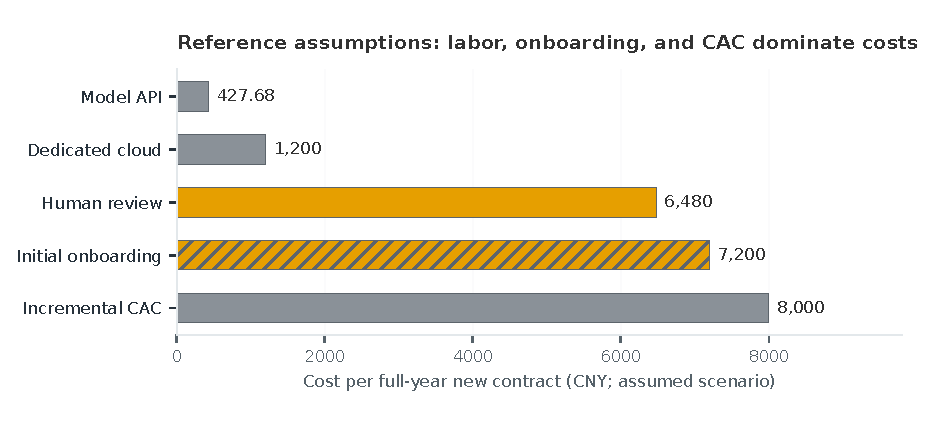
\includegraphics[width=\linewidth]{../../assets/en/business-costs.pdf}
\caption{Baseline assumed costs per full-year contract. API is an external price times assumed usage. Labor, setup, cloud, and acquisition are planning inputs; fixed company costs are separate.}\label{fig:concise-business-costs}
\end{figure}\FloatBarrier

\begin{table}[htbp]\centering\small
\caption{Baseline and joint stress assumptions. Amounts are CNY per full-year new contract; complete inputs and the efficiency scenario remain in supplementary data.}\label{tab:concise-business-finance}
\begin{tabularx}{\linewidth}{@{}Yrr@{}}\toprule
Item & Baseline & Joint stress\\\midrule
Price/enrolment; turns/enrolment &120; 120&90; 180\\
Review proportion; minutes/review &2\%; 3&5\%; 5\\
Annual revenue &72000&54000\\
Delivery cost &15307.68&54072\\
Incremental acquisition &8000&15000\\
Contribution after delivery/acquisition &48692.32&$-15072$\\\bottomrule
\end{tabularx}
\end{table}\FloatBarrier

Baseline delivery comprises CNY 427.68 API, 6480 review, 7200 setup, and 1200 cloud. Direct contribution margin before acquisition is 78.74\%. Joint stress also uses 120 setup hours and CNY 1800 cloud. Expansion cannot repair its negative contribution. Annual fixed spending assumes CNY 600000 (50000/month, including 42000 personnel). It needs 13 baseline full-year contracts, or 15 including CNY 100000 startup cost; this static calculation is not the first year with staggered starts. No scenario probabilities, lifetime value, or renewal forecast are inferred.

\begin{figure}[htbp]\centering
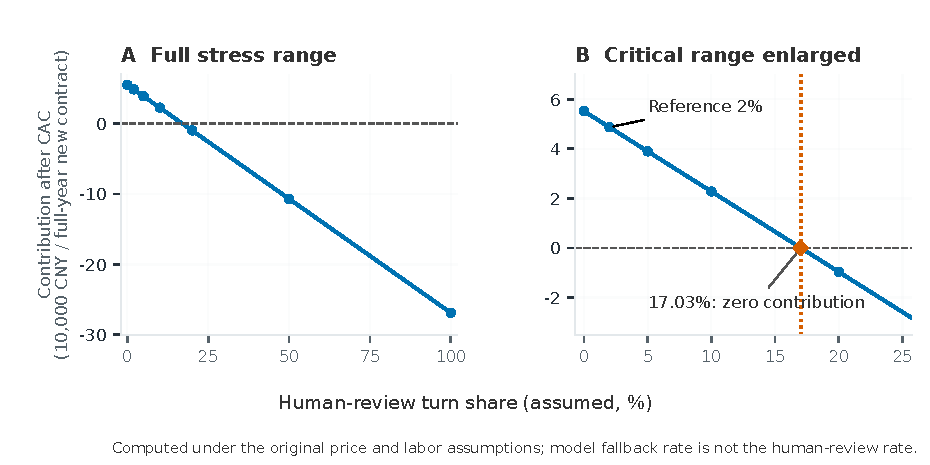
\includegraphics[width=\linewidth]{../../assets/en/business-review-stress.pdf}
\caption{Manual-review sensitivity holding other baseline assumptions fixed. The zero-contribution point near 17.03\% is commercial capacity, not an acceptable quality threshold or an observed review rate.}\label{fig:concise-business-review}
\end{figure}\FloatBarrier

At 10\%, 20\%, and 50\% review, annual contributions are CNY 22772.32, $-9627.68$, and $-106827.68$. Model non-adoption or fallback frequency cannot be converted into business review probability. If required quality costs more than the 17.03\% break-even burden, raise price, narrow scope, or stop productization; quality protection must not be lowered to meet margin.

\subsection{Cash plan and simulated funding}
A simulated CNY 1 million raise supports 12 months of engineering/pilot/procurement validation, without an asserted valuation or exit return. Annual contracts start in months 4, 7, and 10, invoice at activation, and pay three months later. Revenue is spread over service months for planning, not formal accounting. The plan includes CNY 100000 initial spending, 50000/month fixed costs, and activation-linked integration/acquisition plus usage. Actual acquisition expenditure may occur earlier than this simplified timing.

\begin{figure}[htbp]\centering
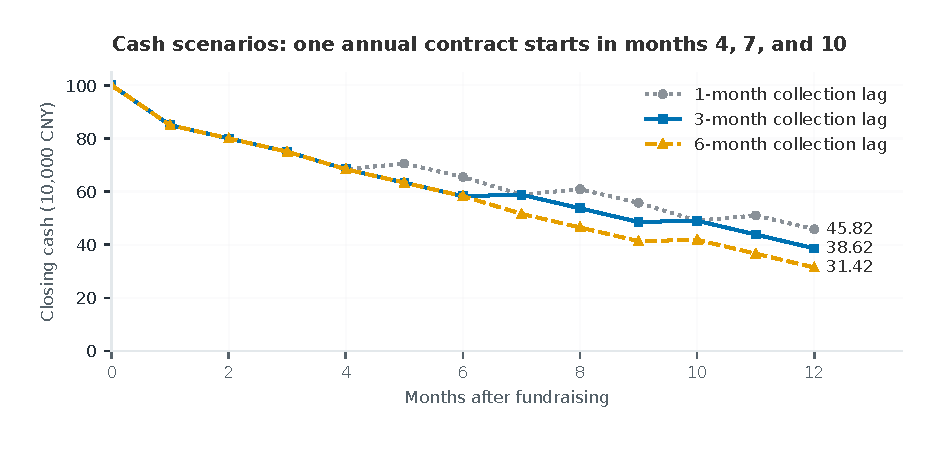
\includegraphics[width=\linewidth]{../../assets/en/business-cash.pdf}
\caption{Cash under one-, three-, and six-month collection lags, starting with assumed CNY 1 million funding. Contract starts and collections have not occurred.}\label{fig:concise-business-cash}
\end{figure}\FloatBarrier

The three-month baseline yields CNY 108000 allocated first-year revenue, 144000 receipts, and 216000 year-end annualized contracts. Approximately 757800 cash spending leaves 386200; the month-10 contract pays in year 2. Remaining cash funds future delivery and is not profit. Tax, financing, bad debt, refunds, and hardware are excluded. Local the agent study runtime does not establish production latency or cloud capacity. Pilot delay requires a revised cash plan.

\section{Validation gates and decision}
The next step is a supervised pilot conditional on further content checks, rather than automatic progression to selling. Engineering repair of known C08/S02 inputs is complete; independent teacher review, student learning evaluation, and procurement remain pending.

\begin{table}[htbp]\centering\small
\caption{Proposed evidence collection and release conditions; these are plans, not achieved outcomes.}\label{tab:concise-business-gates}
\begin{tabularx}{\linewidth}{@{}p{29mm}Y@{}}\toprule
Stage & Evidence and decision boundary\\\midrule
Content verification & New independent questions and 100 blinded teacher reviews; zero severe errors for release, with immediate pause for serious misleading feedback, unauthorized action, or memory contamination.\\
Course pilot & Two courses/about 100 voluntary learners; randomize within courses where feasible, count all preparation/review/correction/maintenance work, and test unaided transfer two weeks later with blinded grading. This sample estimates feasibility/variance, not guaranteed power.\\
Quality and workload & Proposed misleading rate $\leq2\%$, net time saving $\geq20\%$, and post-test difference versus control no worse than $-5$ points on a 100-point scale. Pre-register analysis and report intervals; an interval crossing a gate means uncertainty. Zero misleading responses in 100 independent items gives a one-sided 95\% upper bound of 2.95\%; supporting the 2\% error-rate gate requires at least 149 independent items with no misleading response. Repeated items from the same learner may not be independent.\\
Purchase and delivery & Interview 15 teachers/five procurement roles; record current workflow before demonstration, refusals, quotations, signing, invoicing, and receipts separately. Three expressions of interest are a target, not three customers.\\\bottomrule
\end{tabularx}
\end{table}\FloatBarrier

A 20\% time saving covers the assumed fee through labor value alone only if baseline work is at least 400 minutes/enrolment; this workload has not been measured. Otherwise pricing needs revision or separately evidenced benefits. Severe events are tracked separately from average error rates. A pilot needs teacher-agreed gates, contamination/withdrawal records, and a control using existing support. Team needs are engineering, curriculum evaluation, and customer delivery; no recruited team or school partnership is implied.

Future handling of learner identifiers and error histories requires a processing basis, minimized fields, retention limits, correction/deletion, commissioned-processing responsibilities, and applicable impact assessment~\cite{businesspipl}. Proposed pseudonyms, course access, and correction audits are not implemented compliance certification. Production additionally requires execution isolation, concurrency/security tests, supplier/version control, and verified procurement/data terms. Free substitutes, adaptation labor, delays, and renewals remain commercial risks. If only intensive human service is reliable, it must be priced honestly as such; negative contribution is a stopping condition.

The evidence supports bounded preparation for supervised validation, not autonomous tutoring, competitive superiority, or proven willingness to pay. Full source snapshots, 21-source ledger, three financial scenarios, 25 sensitivity combinations, monthly cash, interview/review forms, and calculation code remain under \path{business/} and \path{business/validation/}. 
\FloatBarrier
\begin{thebibliography}{99}
% report opens the bibliography with \chapter*. hyperref sets the heading's
% destination there; writing the entry now keeps the TOC link on that page.
\addcontentsline{toc}{chapter}{\bibname}
\small
\setlength{\itemsep}{4pt}

\bibitem{nat}
Yang Li, Youssef Emad, Karthik Padthe, et~al.
\href{https://arxiv.org/abs/2507.01921v1}{NaturalThoughts: Selecting and Distilling Reasoning Traces for General Reasoning Tasks}.
arXiv:2507.01921v1, 2025.

\bibitem{matrix}
Dong Wang, Yang Li, Ansong Ni, et~al.
\href{https://arxiv.org/abs/2511.21686v2}{Matrix: Peer-to-Peer Multi-Agent Synthetic Data Generation Framework}.
Conference on Machine Learning and Systems (MLSys), 2026. This report uses arXiv:2511.21686v2.

\bibitem{air}
Bingxiang He, Wenbin Zhang, Jiaxi Song, et~al.
\href{https://openreview.net/pdf?id=Sz3ZU6oeVJ}{AIR: A Systematic Analysis of Annotations, Instructions, and Response Pairs in Preference Dataset}.
Conference on Language Modeling (COLM), 2025.

\bibitem{easy}
ConardLi and contributors.
\href{https://github.com/ConardLi/easy-dataset}{Easy Dataset}.
GitHub repository, accessed 4 November 2026.

\bibitem{dataflow}
OpenDCAI and contributors.
\href{https://github.com/OpenDCAI/DataFlow}{DataFlow}.
GitHub repository, accessed 4 November 2026.

\bibitem{trl}
Hugging Face.
\href{https://huggingface.co/docs/trl/en/dataset_formats}{Dataset formats and types}.
TRL documentation, accessed 4 November 2026.

\bibitem{fdpo}
Tetsuro Morimura, Mitsuki Sakamoto, Yuu Jinnai, Kenshi Abe, and Kaito Ariu.
\href{https://aclanthology.org/2024.emnlp-main.1266/}{Filtered Direct Preference Optimization}.
Proceedings of EMNLP, 2024, pp.~22729--22770.

\bibitem{rethink}
Ziche Liu, Rui Ke, Yajiao Liu, Feng Jiang, and Haizhou Li.
\href{https://aclanthology.org/2025.naacl-long.336/}{Take the Essence and Discard the Dross: A Rethinking on Data Selection for Fine-Tuning Large Language Models}.
Proceedings of NAACL, Volume~1: Long Papers, 2025, pp.~6595--6611.

\bibitem{deita}
Wei Liu, Weihao Zeng, Keqing He, Yong Jiang, and Junxian He.
\href{https://openreview.net/forum?id=BTKAeLqLMw}{What Makes Good Data for Alignment? A Comprehensive Study of Automatic Data Selection in Instruction Tuning}.
International Conference on Learning Representations (ICLR), 2024.

\bibitem{learnlm}
Irina Jurenka, Markus Kunesch, Kevin R.~McKee, et~al.
\href{https://arxiv.org/abs/2407.12687v4}{Towards Responsible Development of Generative AI for Education: An Evaluation-Driven Approach}.
arXiv:2407.12687, 2024. The supplied v4 revision is used.

\bibitem{edu_survey}
Shen Wang, Tianlong Xu, Hang Li, et~al.
\href{https://arxiv.org/abs/2403.18105v2}{Large Language Models for Education: A Survey and Outlook}.
arXiv:2403.18105v2, 2024.

\bibitem{agent_survey}
Zhendong Chu, Shen Wang, Jian Xie, et~al.
\href{https://aclanthology.org/2025.findings-emnlp.743/}{LLM Agents for Education: Advances and Applications}.
Findings of the Association for Computational Linguistics: EMNLP 2025, pp.~13782--13810.
The supplied local version is \href{https://arxiv.org/abs/2503.11733v2}{arXiv:2503.11733v2}, revised 2026.

\bibitem{simclass}
Zheyuan Zhang, Daniel Zhang-Li, Jifan Yu, et~al.
\href{https://aclanthology.org/2025.naacl-long.520/}{Simulating Classroom Education with LLM-Empowered Agents}.
Proceedings of NAACL, Volume~1: Long Papers, 2025, pp.~10364--10379.

\bibitem{qwenbase}
Qwen Team. \href{https://huggingface.co/Qwen/Qwen2.5-0.5B}{Qwen2.5-0.5B: Base model card}. Official pretrained model and tokenizer configuration. \href{https://modelscope.cn/models/Qwen/Qwen2.5-0.5B}{official ModelScope repository}.

\bibitem{lora}
Edward J. Hu, Yelong Shen, Phillip Wallis, et al.
\href{https://arxiv.org/abs/2106.09685}{LoRA: Low-Rank Adaptation of Large Language Models}. ICLR 2022.

\bibitem{dpo}
Rafael Rafailov, Archit Sharma, Eric Mitchell, et al.
\href{https://arxiv.org/abs/2305.18290}{Direct Preference Optimization: Your Language Model is Secretly a Reward Model}. NeurIPS 2023.
\bibitem{openmaic}
THU-MAIC. \href{https://github.com/THU-MAIC/OpenMAIC/tree/5bd8cc840ee6397d063e1fe6aba974b9f0401593}{OpenMAIC: Open Multi-Agent Interactive Classroom}. GitHub repository, pinned commit \texttt{5bd8cc840ee6} (6 November 2026), accessed 7 November 2026. Full commit and file hashes:  \filepath{tutor/legacy/research/source_manifest.json}.

\bibitem{businesscambridge} Accelerate Cambridge. \href{https://www.jbs.cam.ac.uk/wp-content/uploads/2020/08/how-to-write-a-business-plan.pdf}{How to write a business plan}. Cambridge Judge Business School, October 2013. Business-plan reference supplied in the course specification.
\bibitem{businessmoe} Ministry of Education of the People's Republic of China. \href{https://www.moe.gov.cn/jyb_sjzl/sjzl_fztjgb/202607/t20260706_1442870.html}{Statistical Bulletin on National Education Development in 2025}. 6 July 2026. Cross-checked against the \href{https://jyt.hlj.gov.cn/jyt/c110518/202608/c00_31969727.shtml}{official Heilongjiang education-department republication}.
\bibitem{businesskestin} Greg Kestin, Kelly Miller, Anna Klales, Timothy Milbourne, Gregorio Ponti. \href{https://doi.org/10.1038/s41598-025-97652-6}{AI tutoring outperforms in-class active learning: an RCT introducing a novel research-based design in an authentic educational setting}. Scientific Reports 15, 17458, 2025. \href{https://pmc.ncbi.nlm.nih.gov/articles/PMC12179260/}{full text at PMC}.
\bibitem{businessbastani} Hamsa Bastani, Osbert Bastani, Alp Sungu, et al. \href{https://doi.org/10.1073/pnas.2422633122}{Generative AI without guardrails can harm learning: Evidence from high school mathematics}. PNAS 122(26), e2422633122, 2025. \href{https://pmc.ncbi.nlm.nih.gov/articles/PMC12232635/}{full text at PMC}.
\bibitem{businesscodeaid} Majeed Kazemitabaar, Runlong Ye, Xiaoning Wang, et al. \href{https://arxiv.org/abs/2401.11314v2}{CodeAid: Evaluating a Classroom Deployment of an LLM-based Programming Assistant that Balances Student and Educator Needs}. CHI 2024, DOI: 10.1145/3613904.3642773. The supplied arXiv v2 was checked.
\bibitem{businesscgprice} CodeGrade. \href{https://www.codegrade.com/pricing}{Pricing \& Plans}. Official dynamic pricing page, accessed 7 November 2026. Original units retained; not an institutional contract quote.
\bibitem{businesscgai} CodeGrade. \href{https://www.codegrade.com/solutions/ai-assistant}{AI Coding Assistant for CS Courses}. Official product description, accessed 7 November 2026.
\bibitem{businesscghelp} CodeGrade. \href{https://help.codegrade.com/setup-assignment/other-features/ai-assistant}{AI Assistant}. Official documentation, accessed 7 November 2026; the archived page retains a Beta description.
\bibitem{businesscgrelease} CodeGrade. \href{https://www.codegrade.com/blog/codegrade-snowball-miracle-release}{Snowball Miracle: A Terminal, a Smarter AI Assistant, and Tighter Exam Controls}. 25 September 2026; accessed 7 November 2026.
\bibitem{businesskhanprice} Khan Academy. \href{https://khanmigo.ai/pricing}{Khanmigo pricing}. Official dynamic pricing page, accessed 7 November 2026.
\bibitem{businesskhan} Khan Academy. \href{https://khanmigo.ai/}{Khanmigo: AI-powered teaching assistant \& tutor}. Official product and FAQ, accessed 7 November 2026.
\bibitem{businesskhangeo} Khan Academy. \href{https://blog.khanacademy.org/teachers-in-44-countries-now-get-free-access-to-khanmigo-in-english-thanks-to-microsoft-support/}{Khanmigo for Teachers Now Available in Pilot in 180+ Countries, Powered by Microsoft}. Initially published 17 July 2024, explicitly updated 4 December 2025; accessed 7 November 2026.
\bibitem{businessstudymode} OpenAI. \href{https://help.openai.com/en/articles/11780217-using-study-mode-in-chatgpt}{Using study mode in ChatGPT}. Official help page, accessed 7 November 2026; availability and limits depend on plan, region and updates.
\bibitem{businessprice} Alibaba Cloud. \href{https://help.aliyun.com/zh/model-studio/qwen-plus}{qwen-plus model information}. China North 2 (Beijing), input up to 128k, real-time non-thinking list price; accessed 7 November 2026. No discount or teaching-effect claim.
\bibitem{businesspipl} Standing Committee of the National People's Congress. \href{https://www.cac.gov.cn/2021-08/20/c_1631050028355286.htm}{Personal Information Protection Law of the People's Republic of China}. Adopted 20 August 2021, effective 1 November 2021; CAC republication, accessed 7 November 2026.

\end{thebibliography}

\appendix
\chapter{Evidence and Reproducibility}\label{app:repro}\section{Published evidence and reproduction}
The repository provides source, frozen educational datasets, saved responses and per-item reviews. Numerical results are not regenerated by this report build. Official model weights, adapter/optimizer binaries and local runtime environments are excluded; rerunning models requires the pinned official base and the documented dependencies. Inspecting saved outputs requires no model execution.
\begin{table}[htbp]\centering\small
\caption{Research evidence and code entry points.}
\begin{tabularx}{\linewidth}{@{}p{30mm}Y@{}}\toprule
Area & Published entry points\\\midrule
Data synthesis & \filepath{synthesis/}: generator, frozen 1000-example SFT and 500-pair preference release, candidate ledger and validation. \filepath{synthesis_legacy/} and \filepath{data/legacy/} retain the earlier filtering comparison.\\
Post-training & \filepath{training/}: SFT/DPO and evaluation code, first cloud run, exploratory retry, continued-SFT control, full answer comparisons, initial failed numerical audit and its separate review.\\
Learner memory & \filepath{tutor/}: original frozen cases, repaired/structured controllers, raw role responses, memory evidence, tool regressions and the isolated rendering correction.\\
Feasibility & \filepath{business/}: sources, assumptions, unit economics, sensitivity and conditional validation plans.\\
Figures & \filepath{reports/assets/}: vector scientific figures and conceptual artwork. The artwork is explanatory, not a measured result.\\\bottomrule
\end{tabularx}\end{table}\FloatBarrier
English quotations translate the original Chinese recorded responses; they are not a new English-language evaluation. Complete saved answers remain the basis for factual review. Published records have identifying and local-machine fields removed; original scientific values and failure labels are retained. Historical run checksums describe original artifacts, while the release manifest identifies the published files.

The repository's bilingual instructions provide dependency setup, saved-record verification, a model-free controller smoke check, and optional model-training commands. PDF building requires Tectonic or a compatible XeLaTeX engine and the documented fonts. A runnable workflow is not evidence of reliable autonomous teaching or of real-student learning gains.
\FloatBarrier
\chapter{Research Provenance and Limitations}\label{app:prompts}\section{Assistance and evidence boundaries}
OpenAI Codex/GPT-6-family assistance supported research, code, review, translation and figure design. The studied model is the official Qwen2.5-0.5B base and its recorded adapters. A separately sourced same-size Instruct checkpoint is diagnostic and is not a training outcome. Rule-based synthesis did not invoke a teacher model per sample. Reviews are same-project, non-blind technical checks rather than independent teacher evaluation.

Research role templates and instrumented model inputs accompany the relevant controllers and saved traces. Personal conversations and internal delegation history are excluded from this anonymized research release; it makes no claim to provide complete authoring history. Editable code generated the scientific schematics. OpenAI image generation produced the unlabelled conceptual cover artwork; its exact generation-model identifier was not returned.

\section{Limitations}
The data cover a restricted Python subset with repeated templates and coupled preference reasons. Small, same-author development and evaluation sets, one training seed, exploratory test reuse, and unmatched control token budgets limit causal claims. Larger-model and controlled data ablations were not run. Reference NLL, parser success and fallback correctness do not measure learning. The system trusts caller-supplied learner identifiers and lacks production authentication. Real-student gains, teacher workload savings, institutional demand and willingness to pay remain unmeasured. Failed outputs, the original numerical exception and unsuccessful remediation are retained.

\end{document}
